\documentclass[a4paper,12pt]{article} 

% packages and main settings
\usepackage[left=3cm, right=2cm, top=2cm, bottom=2cm]{geometry}
\usepackage[english]{babel}    
\usepackage[utf8]{inputenc}  
\usepackage[T1]{fontenc}        
\usepackage{lmodern}            
\usepackage{microtype}          
\usepackage{amsmath}
\usepackage{amsfonts, amsthm, amssymb, graphicx, booktabs}
\usepackage{bm} %bold epsilon
\usepackage{newclude}   
\usepackage{placeins}  %surpresses floating tables
\usepackage[labelfont=bf]{caption} %Figure etc steht dann in small caps 
\usepackage[labelsep=period]{caption} % dot after figure, table caption.
\usepackage[flushleft]{threeparttable} % for notes below table
\usepackage{multirow} % for table cell merge along rows
\usepackage{graphicx} % to adjust tablesize to textwidth
\usepackage{caption}  % for centered captions
\usepackage{float} % to set of autopositioning of tables
\usepackage[bottom,hang,flushmargin]{footmisc} % forces footnotes to the bottom
\usepackage{setspace}           % Fuer 1.5 fachen Zeilenabstand  
\onehalfspacing % 1.5 cm Zeilenabstand
%Bibtex
\usepackage[round,sort&compress]{natbib}
 
\bibliographystyle{chicago} % chicago bib style like in AER
\usepackage[hidelinks]{hyperref} % fuer links und verweise. Cleverref ist eigentlich besser. 


% Create header. The header must be surpressed for 
% every first page per section and a solution
% for the Appendix is used in the respective subfile.
\usepackage{fancyhdr}
\pagestyle{fancy}
\fancyhf{}
\chead{\nouppercase{\textit{\leftmark}}}
\cfoot{\thepage}
\renewcommand{\headrulewidth}{0pt} % no vertical line

%\usepackage{lipsum}  % check if formats work

\usepackage{afterpage} %clearpage w/o pagebreak for "header bug"

% Expectation symbol
\DeclareMathOperator*{\E}{\mathbb{E}}

 % thin space, limits underneath in displays
% for strike through
\DeclareMathOperator*{\argmax}{argmax}
\newcommand*{\defeq}{\stackrel{\text{def}}{=}}
\usepackage[normalem]{ulem}
% try to use strikeout in section headers and others
\DeclareRobustCommand{\hsout}[1]{\texorpdfstring{\sout{#1}}{#1}}

% for gray table row color
\usepackage[table]{xcolor}

% decimal dot alignment in table columns
\usepackage{siunitx}

% for footnotes in table
\usepackage[flushleft]{threeparttable}

% for underbar
\newcommand{\ubar}[1]{\text{\b{$#1$}}}

\usepackage{tikz}

% Setup for urls
\usepackage{url}

\defcitealias{Respy-Stenzel.2019}{\textit{respy}}
\defcitealias{Gabler.2019}{\textit{estimagic}}
\defcitealias{Stenzel.2020}{\textit{Master's Thesis Replication Repository}}
\defcitealias{NLSY79}{NLSY79}


\begin{document}


\begin{titlepage}
	
\begin{center}
	
\vspace*{1.0cm}

{\LARGE
\bfseries Uncertainty Quantification for an \\
\vspace*{0.5cm}
Eckstein-Keane-Wolpin model
}
\\
\vspace*{0.5cm}
{\LARGE
\bfseries with correlated input parameters
}

{\large
\vspace*{4.0cm}
Master Thesis Presented to the\\
\vspace*{0.25cm}
Department of Economics at the\\
\vspace*{0.25cm}
Rheinische Friedrichs-Wilhelm-Universität Bonn\\

\vspace*{2.0cm}
in Partial Fulfillment of the Requirements of the Degree of\\
\vspace*{0.25cm}
Master of Science (M.Sc.)\\

\vspace*{4.0cm}
Supervisor: Prof. Dr. Philipp Eisenhauer\\

\vspace*{2.0cm}
Submitted in January 2020 by:\\
Tobias Stenzel\\
Matriculation Number: 2971049
}

\end{center}

\end{titlepage}
\newpage

\thispagestyle{plain} % no header on first page
\tableofcontents
\newpage

\setcounter{page}{1}
\pagenumbering{Roman}


% no section command to prevent "A" before "Appendix" in toc.

\addcontentsline{toc}{section}{Abbreviations} 

\section*{Abbreviations} % no number before Appendix in toc
\thispagestyle{plain} % surpress header on first page

\phantom{This text will be invisible} 
\hspace{20cm}



% Please add the following required packages to your document preamble:
% \usepackage{booktabs}
\begin{table}[H]
	\centering
	\renewcommand{\arraystretch}{1.2}%
	\begin{tabular}{@{}ll@{}}
		\toprule
	Term\phantom{space}	& Meaning \\ \midrule
			$\bold{cdf}$	& Cumulative distribution function \\
		$\bold{EE}$	& Elementary Effect \\
	$\bold{GSA}$	& Global sensitivity analysis \\
	$\bold{i.i.d.}$	& Independent and identically distributed  \\
	$\bold{LSA}$	& Local sensitivity analysis \\
    $\bold{QoI}$	& Quantity of interest \\
    $\bold{UQ}$	& Uncertainty quantification \\
    $\bold{USD}$	& US-Dollar  \\
 \bottomrule
	\end{tabular}
\end{table}
\newpage
\addcontentsline{toc}{section}{List of Figures} 

%\section*{List of Figures} % no number before LoFs in toc
\thispagestyle{plain} % surpress header on first page

\listoffigures
\newpage
\addcontentsline{toc}{section}{List of Tables} 

%\section*{List of Tables} % no number before LoTs in toc
\thispagestyle{plain} % surpress header on first page

\listoftables
\newpage

\setcounter{page}{1}
\pagenumbering{arabic}

\section{Introduction}
\thispagestyle{plain} % surpress header on first page

How certain is a model outcome? This question is the subject of the mathematical field of uncertainty quantification (UQ). It is hard to find an area that is untouched by uncertainty. Therefore, all kinds of agents, but especially decision-makers and researchers, would benefit largely from a better understanding of uncertainties. For economic studies, the need for UQ  has been identified for quite some time (\cite{Hansen.1996}; \cite{Canova.1994}; \cite{Kydland.1992}). However, the economic research practice has not evolved accordingly (\cite{Harenberg.2019}).\\

\noindent
This thesis' objective is to quantify the parametric uncertainty of the occupational choice model by \cite{Keane.1994} (KW94) which belongs to the class of Eckstein-Keane-Wolpin models (\cite{Aguirregabiria.2010}). Assuming that the model parameters are estimated, the parametric uncertainty refers to the impact of the computed standard errors on the variation of the model outputs. I estimate the parameters from simulated data.
The uncertain model output, or quantity of interest (QoI), is the effect of a 500 US-Dollar (USD) subsidy on annual tuition costs for higher education on the average years of education. The UQ is divided into two parts. The first part deals with the general uncertainty of the QoI that is caused by all parameters together. The second part tries to identify the parameters that do not influence the QoI.\\

\noindent
I find the following result for the general uncertainty: The mean QoI is an increase of 1.5 years in average education. The QoI's uncertainty is relatively low with 0.1 years.\\

\noindent
The second part does not provide clear results. This is due to two properties of the KW94 model.
The first property is that the model is rather complex and large, with 27 input parameters. Therefore, the computation time prohibits me from selecting the most conclusive measures.
The second property is that the model parameters are correlated.


For a model with these properties, I find that only the work by \cite{ge2014efficient} potentially includes measures that are suited to the model. These measures base on Elementary Effects (EEs) that are computed based on random samples that follow specific patterns (\cite{Morris.1991}; \cite{saltelli2010variance}). An EE is defined as the local derivative of a function with respect to one argument. The EE does not assume that the change in the argument is infinitesimally small. The analysis of the measures by \cite{ge2014efficient} reveals that they can lead to arbitrary parameter rankings. However, building on their work, I develop redesigned measures and demonstrate that they can precisely apportion the parametric uncertainty for a linear test function with correlated input parameters.

Nonetheless, I am not able to develop recommendations about which parameters to fix. The reasons are twofold, and they are not specific to correlated functions but specific to EE-based measures in general. First, it is unclear which EE-based measures to use. Conceptually, the EE can quantify the effect of the uncertainty of one parameter on the level of a QoI. However, the effect of EE-based measures on the variation of a QoI is not well-understood. Therefore, there is no consensus about which measure to use (\cite{campolongo2007effective}; \cite{kucherenko2009derivative}; \cite{Smith.2014}). Yet, I find some evidence that sigma-normalised EEs can lead to sensible results.
Second, the literature does not develop convincing cut-off criteria for declaring a parameter non-influential.

An additional result is that there is a high variance between the EEs computed from the data generated by two different sampling schemes. These schemes are the trajectory and radial design. They differ in their pattern to generate the changes in the function arguments that are necessary for computing the local derivatives. The results indicate that these changes are too large to capture the variation of the KW94 model. This finding is in line with \cite{kucherenko2009derivative}.\\

\noindent
The structure of this thesis is as follows. I introduce the UQ framework and present the most important concepts in section 2. I review the applications of UQ in the economic literature in section 3. The following section reviews the EEs for correlated input parameters in \cite{ge2017extending} and develops the redesigned EEs. I also demonstrate my ability to replicate their results, and I validate my conceptual analysis of their measures as well as the redesigned measures with a linear test function. Section 5 introduces the occupational choice model by \cite{Keane.1994} and presents the estimation results of the input parameters. Section 6 shows the results for the UQ. Section 7 discusses the findings and identifies topics for future research. Section 8 concludes.






\newpage

\section{Uncertainty Quantification Framework}
\thispagestyle{plain} % surpress header on first page

This section consists of three parts. The first part gives an overview of uncertainty quantification and introduces the basic notation. The following two parts explain the more involved UQ measures that are computed in this thesis.
The second part describes Morris screening. It is a method used to decrease the number of uncertain input parameters thereby reducing the computational burden for the following part.
The third part presents the Sobol' indices. These global measures attribute the variation in the quantity of interest to the uncertainty in individual input parameters. They constitute the thesis' main result.

\subsection{Overview of Uncertainty Quantification}
Model-based forecasting includes two main steps:\footnote{The general procedure of model-based forecasting can also include other steps. However, steps like model validation and model verification can also be viewed as belonging to the analysis of the so-called model uncertainty. The concept of model uncertainty is briefly explained in the next paragraph.} The first step is the calibration. In this step, the input parameters of the model are estimated. The second step is the prediction. The prediction contains the evaluation of model at the estimated parameters to make statements about the future. These statements are made in a probabilistic way. Thereby, the uncertainty of these statements is emphasised.\\
\newline
There are four sources of uncertainty in modern forecasts that are based on complex computational models. The first source, the model uncertainty, is the uncertainty of whether the mathematical model represents the reality appropriately.\footnote{However, It seems that there are not many powerful instruments to evaluate and improve the model uncertainty except comparing statements derived from the model to the data and then improving it where appropriate.} The second source, the input uncertainty, is the uncertainty about the size of the input parameters of the model. The third one, the numerical uncertainty, comes from potential errors and uncertainties introduced by the conversion from a mathematical to a computational model. The last source of uncertainty, the measurement uncertainty, is the accuracy of the experimental data that is used to approximate and calibrate the model.

The thesis deals with the second source of uncertainty, the input uncertainty. In my view, this is the source for which uncertainty quantification offers the most instruments and also the strongest instruments. This results from the fact that the estimation step yields basic measures for the variability or uncertainty in the input parameter estimates. These can then be used to compute a wide variety of measures for the input uncertainty.\\
\newline
The following explains the basic notation for the quantification of the input uncertainty. An essential step is to define the quantity that one wants to predict with a model. This quantity is called the quantity of interest (henceforth QoI) and denoted by $q$. For instance, the QoI in the thesis is the impact of a 500 USD tuition subsidy for higher education on average schooling years. The uncertain model parameters are denoted by vector $\pmb{\theta}$. The function that computes QoI $q$ by evaluating a computation model and, if necessary, post-processing the model output is denoted by $\mathcal{M}$. Thus,
\begin{align}
q = \mathcal{M}(\pmb{\theta}).
\end{align}
Large-scale UQ applications draw from various disciplines like probability, statistics, analysis, and numeric. They are used in a combined effort for parameter estimation, surrogate model construction, parameter selection, uncertainty propagation, LSA, and GSA, amongst others. 

Parameter estimation covers the calibration step. There is a large number of estimation techniques for various types of models. The thesis uses a maximum likelihood approach detailed in the Model and Estimation section. However, the parameter estimation is not the main focus. 


If the run time of a model is too long to compute some UQ measures, surrogate models are constructed to substitute the original model $\mathcal{M}$. These surrogate models are functions of the model input parameters that are faster to evaluate. They are also called interpolants because these functions are computed from a random sample of input parameter vectors drawn from the input distribution and evaluated by the model. Therefore, evaluations of the surrogate model interpolate this sample. Some techniques yield functions that have properties which simplify the computation of some UQ measures tremendously.

Another way to reduce computation, not necessarily of the model, but of UQ measures, is to reduce the number of uncertain input parameters as part of parameter selection. This is the approach that the thesis takes instead of the construction of a surrogate model.\footnote{Further remarks on the choice of measures and methods are discussed at the end of the literature review. This sequence allows for direct comparisons with other contributions.} The chosen technique is called Morris sampling and detailed in the following Global Sensitivity Analysis subsection.

Uncertainty propagation is the core of the prediction step. It comprises the construction of the QoI's probability distribution by propagating the input uncertainty through the model. For instance, this can be achieved by repeatedly evaluating a sample of random input parameters by the model (as also required for the construction of a surrogate model). Uncertainty propagation also involves the computation of descriptive statistics like the probabilities for a set of specific events in the QoI range using this distribution. This is conceptually simple. The results are presented in the Uncertainty Propagation section. The construction of the probability distribution is also important for designing the subsequent steps like a sensitivity analysis. For example, if the distribution is unimodal and symmetric variance-based UQ measures are meaningful. If the distribution has a less tractable, for instance a bimodal shape, density-based measures are better suited.

In UQ, sensitivity analysis has the objective of quantifying the relative contribution of the uncertainty in individual input parameters to the total uncertainty in the QoI. Moreover, it answers the question of how variations in parameters affect QoI responses. The thesis focuses on the first part because the range of the QoI's distribution has no particularly critical interval. If the results of a sensitivity analysis suggest that a parameter's contribution to the QoI's is negligible, this parameter can be fixed. These fixings simplify subsequent parameter estimations and uncertainty propagations. Therefore, these analyses can be applied alternately. Sensitivity analyses can be local or global.

Local sensitivity analysis is the most frequently used level of sensitivity analysis in the literature of most scientific disciplines. It provides measures for the above objectives by changes of input parameter values about some nominal values at specific choices of local points in the input parameter space. The two choices, the nominal value that changes the input parameters and the local point at which to change the parameters, contain a degree of arbitrariness. This arbitrariness can yield false results if the model is non-linear and does contain interactions between the input parameters. These limitations can be overcome in a global sensitivity analysis (henceforth GSA) as presented in the next subsection.\\
\newline
Beforehand, a vital remark is made in anticipation of the estimation results for the input parameters' uncertainty: In realistic models, the estimates for the input parameters tend to be correlated. Therefore, the measures and methods in the next section are presented with their respective extensions that allow for correlated input parameters. These extensions are published in contributions from the last 15 years. Therefore, they are relatively novel.

In general, the emphasis on UQ measures for models with correlated input parameters in the literature is not particularly strong.
This has the following reason: For correlated input parameters with a known, tractable joint distribution function like, for instance, the normal distribution, sampling-based measures can be computed by sampling from the unit cube. The samples are then converted from the unit cube to the domain of the joint probability distribution by evaluating the draws with the inverse cumulative distribution function, thereby accounting for the correlation. Alternatively, the decorrelation techniques Rosenblatt and Nataf transformation are usually used for less simple distribution functions



\subsection{Global Sensitivity Analysis}
\subsubsection{Morris Screening}
\cite{Morris.1991}

\cite{Saltelli.2008}

\cite{lemaire2013structural}
\cite{gentle2006random}
\cite{ge2017extending}
\cite{ge2014efficient}
\cite{campolongo2007effective}
\cite{Smith.2014}
\subsubsection{Sobol' Indices}

\begin{align}
S_i = \frac{\text{Var}_i[Y|X_i ]}{\text{Var}[Y]}
\end{align}

\begin{align}
S_i = \frac{\text{Var}_i[\E_{\sim i}[Y|X_i ]]}{\text{Var}[Y]}
\end{align}

\begin{align}
S_{ij} = \frac{\text{Var}_{ij}[\E_{\sim \{i,j\}}[Y|X_i, X_j ]]}{\text{Var}[Y]} - S_i - S_j
\end{align}

\begin{align}
S_\text{u} = \frac{\text{Var}_\text{u}[\E_{\sim \text{u}}[Y|X_\text{u} ]]}{\text{Var}[Y]} - \sum_{\text{w} \subset \text{u}} S_\text{w}
\end{align}

\begin{align}
S_i^\text{T} = \sum_{i \in \text{u}} S_\text{u}
\end{align}

\begin{align}
\text{Var}[Y] = \text{Var}_i[\E_{\sim i}[Y|X_i]] + \E_{i}[\text{Var}_{\sim i}[Y|X_i]]
\end{align}

\begin{align}
1 = \frac{\text{Var}_i[\E_{\sim i}[Y|X_i]]}{\text{Var}[Y]} + \frac{\E_{i}[Var_{\sim i}[Y|X_i]]}{\text{Var}[Y]}
\end{align}
\begin{align}
1 = S_i + S_{\sim i}^T
\end{align}

\begin{align}
S_{\sim i}^T = \frac{\E_{i}[\text{Var}_{\sim i}[Y|X_i]]}{\text{Var}[Y]}
\end{align}

\begin{align}
S_{i}^T = \frac{\E_{\sim i}[\text{Var}_{i}[Y|X_{\sim i}]]}{\text{Var}[Y]}
\end{align}

\begin{align}
S_\text{u}^{clo} = \frac{\text{Var}_\text{u}[\E_{\sim \text{u}}[Y|X_\text{u} ]]}{\text{Var}[Y]}
\end{align}


\begin{align}
Y = \mathcal{M}(\text{x}) = \mathcal{M}_0 + \sum_{i=1}^{M} \mathcal{M}_i(x_i) + \sum_{1 \leq i \leq j \leq M} \mathcal{M}_{ij}(x_i,x_j) + ... + \mathcal{M}_{12..M}(\text{x})
\end{align}

\begin{align}
S_i = \frac{\text{Cov}[\mathcal{M}_i(x_i), Y]}{\text{Var}[Y]}
\end{align}

\begin{align}
S_i = \frac{\text{Var}[\mathcal{M}_i(x_i)]}{\text{Var}[Y]} + \frac{\text{Cov}[\mathcal{M}_i(x_i)]}{\text{Var}[Y]}
\end{align}

\begin{align}
S_i = \frac{\text{Var}_i[\mathcal{M}_i(x_i)]}{\text{Var}[Y]}
\end{align}

\begin{align}
S_{ij} = \frac{\text{Var}_{ij}[\mathcal{M}_{ij}(x_i,x_j)]}{\text{Var}[Y]}
\end{align}

\begin{align}
\text{Var}[Y] =  \sum_{i=1}^{M} \text{Var}[\mathcal{M}_i(x_i)] + \sum_{1 \leq i \leq j \leq M} \text{Var}[\mathcal{M}_{ij}(x_i,x_j)] + ... + \text{Var}[\mathcal{M}_{12..M}(\text{x})]
\end{align}

\begin{equation}
\begin{aligned}
S_i^T = S_i + \sum_{j \ne i} S_{ij} + \sum_{1 \leq i \leq j \leq M,\{j,k\} \ne i} S_{ijk} + ... = \sum_{i \in \text{w}} S_\text{w} = \\
\frac{1}{\text{Var}[Y]}\sum_{i \in \text{w}} \text{Var}_i[\mathcal{M}_\text{w}(x_\text{w})]
\end{aligned}
\end{equation}

\begin{align}
S_\text{u}^{clo} = \frac{\text{Var}_\text{u}[\mathcal{M}_\text{u}(\text{x}_\text{u})]}{\text{Var}[Y]} +  \sum_{\text{w} \subseteq \text{u}} \frac{\text{Var}_\text{w}[\mathcal{M}_\text{w}(\text{x}_\text{w})]}{\text{Var}[Y]}
\end{align}


\subsection{Surrogate Models and Spectral Expansions}


[Univariate Effects as a measure for comparative statics]

[Philipp: Please add a plot to your thesis (not our notebook) that implements the idea of the uncertainty cone in Figure 1. 2 in our textbook. For example, Figure 1 from KW97 could use such a cone for hte out of support predictions in the occupational shares.]

\newpage
%exlude, just to see how large the next chapter is

\afterpage{\clearpage} % solves problem that header does not disappear in 
% literature review
\section{Uncertainty Quantification in the Economic Literature}
\thispagestyle{plain} % surpress header on first page

The need for UQ as an essential part of quantitative economic studies has long been recognized in the economics profession.\footnote{See \cite{Hansen.1996}, \cite{Kydland.1992} and \cite{Canova.1994}, amongst others.} Also GSA in particular has had strong advocates.\footnote{See \cite{Canova.1995} and \cite{Gregory.1995}.} However, the demanded evolution of research practice has only been met by a few publications until today. This literature review summarizes these publications with regards to two UQ subfields that are emphasized in the prior section. These are uncertainty analysis and quantitative GSA. The review excludes qualitative GSAs because factor fixing is not the objective of the respective publications. A qualitative GSA as a standalone GSA is not considered as best practice (\cite{Saltelli.2004})\footnote{See p. 48.}. Table \ref{tab:lit} gives an overview of the major topics, analyses, measures and methods in the literature.\\

\noindent
I find 14 contributions that meet the described criteria. Arguably, because UQ is more accomplished in climatology, a large share of research comes from climate economics. Another field where UQ finds some application is macroeconomics. Remarkably, no contribution computes their own estimates for the model input uncertainty. The earlier publications tend to use the conceptually simple Monte Carlo uncertainty analysis. However, some prefer Latin hypercube sampling. The idea of Latin hypercube sampling is to improve the speed with which the random draws cover the whole variable range. For this purpose, the range is divided into equally probable intervals. Then, one draws only once from each possible interval combination by discarding further draws of the same combinations. The later contributions focus on GSA. \cite{Harenberg.2019} gives a well-argued explanation about why GSAs are better than LSAs. GSA measures are Sobol' indices, univariate effects and two density-based measures. The majority of papers use surrogate models to save computation time. The recent works use more sophisticated methods like polynomial chaos expansions to construct a surrogate model (as first applied in \cite{Harenberg.2019}) or intrusive approaches (see, for instance, \cite{Scheidegger.2019}). Intrusive methods require essential changes to the model structure, for instance to the state space, whereas the usual non-intrusive methods leave the model untouched and treat it like a so-called black box.\\
\newline
\cite{Harrison.1992} suggest to use uncertainty analysis via Monte Carlo sampling for applied general equilibrium modeling to inspect the uncertainty in model inputs. As a showcase, they propagate the distributions of 48 elasticities through a taxation model by drawing 15,000 input parameter vectors. They analyse their results graphically, using a histogram for their QoI as well as confidence intervals for its mean. For further use, N denotes the size of a Monte Carlo sample.\\
\newline
\cite{Canova.1994} proposes to perform a Monte Carlo uncertainty analysis to reflect upon the calibration of dynamic general equilibrium models. The author also addresses challenges and methods for parameter calibration. \citeauthor{Canova.1994} illustrates his approach by plotting distributions and computing moments and prediction intervals for QoIs in an asset-pricing (N=10,000) and a real business cycle model (N=1,000). Moreover, he analyzes the QoIs' sensitivity towards the uncertainty of individual input parameters by propagating different specifications of input distributions.\\
\newline
More recent examples for Monte Carlo uncertainty analysis investigate climate models, such as \cite{Webster.2012}.
Examples using Latin hypercube sampling are \cite{Mattoo.2009} and \cite{Hope.2006}.\\
\newline
Recently, \cite{Harenberg.2019} compare measures from LSA to measures from GSA for multiple QoIs of the canonical, macroeconomic real business cycle model. Thereby, they provide a context for GSA within UQ. The computed sensitivity measures are Sobol' indices and univariate effects. Univariate effects are the conditional expectation of a QoI as a function of one input parameter $X_i$, where the expectations are taken over $X_{\sim i}$. They are equal to the argument in the variance numerator of the first-order Sobol' index in Equation (\ref{eq:spec_sobol}). The sensitivity indices and univariate effects are obtained by polynomial chaos expansions. For this purpose, \citeauthor{Harenberg.2019} introduce the leave-one-out error estimator as a measure to select an orthogonal polynomial as the surrogate model.

The concept behind this estimator is the following: Take an arbitrary set $A$ of a large number of $n$ input parameter vectors. From this set, create a set $B$ of $n$ sets that contains every possible permutation of set $A$ but leaving out one parameter vector. Then, for each candidate surrogate model specification, first, compute $n$ surrogate models by evaluating each element of set $B$. Second, for each specification, compute the mean of the squared errors between actual and surrogate model evaluated at each element of $B$. This is the leave-one-out error. Finally, one chooses a surrogate model (computed from an arbitrary element of $B$) for the specification with the lowest error.

The authors come to the following conclusion: On the one hand, a LSA can easily be misleading due to the reasons detailed in the previous chapter. LSA methods are typically used in economics. The authors conclude that these are neither adequate for identifying the inputs that drive the uncertainty, nor do they allow to analyse interactions. On the other hand, a GSA can provide profound insights, and polynomial chaos expansions are a fast way to compute approximations for the respective global sensitivity measures.\\
\newline
\cite{Ratto.2008} presents global sensitivity measures for multiple variants of DSGE models computed by Monte Carlo methods and surrogate models. The first measure is density based and derived from the Smirnov test (see, e.g., \cite{Hornberger.1981}): The QoI range is partitioned into a desired set $S$, and an undesired set $\overline{S}$. Then a Monte Carlo sample of parameter vectors from the input distribution is propagated through the model. From the QoI realizations for each set, two cumulative distribution functions for each input parameter, one conditioned on QoI realizations in set $S$, and the other conditioned on realizations in set $\overline{S}$, are generated. For each input independently, it is tested whether the distributions differ. If they do, the parameters and their specific regions that lead to the undesired QoI realizations can directly be identified. The second measure is first-order Sobol' indices. \citeauthor{Ratto.2008} computes them by employing two different surrogate models. The first surrogate is obtained by state-dependent regression. The idea is to regress the QoI on (combinations of) input parameters. The second surrogate is a polynomial representation of the first one. The author finds that the surrogates provide a good fit for the Monte Carlo sample except for the distribution tails. The fit varies conditional on different input parameters. \citeauthor{Ratto.2008} compares his results for the first-order Sobol' indices computed by both surrogates. The results show some differences in size but not in ranking.\\
\newline
\cite{Saltelli.2010} criticise the arbitrary input value choices in the sensitivity analysis design of the influential \cite{Stern.2007} report about the consequences of climate change. Particularly, \citeauthor{Stern.2007} argues that this cost-benefit analysis' results about the economic impact of climate change are robust towards the uncertainty in the input parameters. Yet, \cite{Saltelli.2010} contradict \citeauthor{Stern.2007}'s assertion by presenting a more thorough sensitivity analysis with parameter choices that better represent the original input distribution.\\
\newline
A series of papers (\cite{Anderson.2014}, \cite{Butler.2014}, \cite{Miftakhova.2018}) conducts sensitivity analyses for the dynamic integrated climate-economy model in \cite{Nordhaus.2008}, in short DICE model.  Each work concludes that a GSA is superior to a LSA. Furthermore, all contributions find that leaving some hypothetically low-impact parameters out of the sensitivity analyses lead \citeauthor{Nordhaus.2008} to neglect the uncertainty in important parameters.

\cite{Anderson.2014} use Sobol' indices, the $\delta$-sensitivity measure, and correlation measures for paired QoIs in their GSA. The $\delta$-sensitivity measure (see, e.g., \cite{Borgonovo.2006}) is density-based. It is given by half the expectation value of the absolute difference between the unconditional distribution of a QoI and the QoI distribution conditioned on one specific, fixed input (group). Estimates for these measures are computed with the algorithm used in \cite{Plischke.2013} applied to a Monte-Carlo sample (N=10,000). In \cite{Anderson.2014}, the $\delta$-sensitivity measure is the main measure of sensitivity and used to rank the parameters in terms of their contributions to the model uncertainty. The authors also use a surrogate model obtained through Cut-HDMR (cut-high dimensional model representation; see, e.g., \cite{Ziehn.2009}) for graphical analyses of the interactions between input parameters.

\cite{Butler.2014} also generate importance rankings for the uncertainty in input parameters. However, they use first, second and total order Sobol' indices instead of the $\delta$-sensitivity measure. They compute the Sobol' indices based on Sobol' sequences (\cite{Sobol.1967}) for the results and based on Latin Hypercube sampling (\cite{McKay.1979}) as a check. The results in \cite{Butler.2014} and \cite{Anderson.2014} can not be compared as they analyse different QoIs.

\cite{Miftakhova.2018} applies the GSA procedure outlined by \cite{Harenberg.2019}. The importance ranking that she obtains from the polynomial-chaos-expansions-based Sobol' indices is different from the ranking that \cite{Anderson.2014} obtain from the $\delta$-sensitivity measure. Yet, this is not mentioned by \citeauthor{Miftakhova.2018}.\footnote{I do not have access to the numerical codes. Thus the reasons for the discrepancies remain unclear.} However, the author emphasizes that the standard procedure for obtaining Sobol' indices from a variance decomposition as used by \cite{Anderson.2014} and \cite{Butler.2014} is not feasible for the DICE model because a set of input parameters is calibrated jointly in order to let the model match some observables. Therefore, although these input parameters are not correlated in the classical sense, they are dependent. Hence, the variance-based Sobol decomposition is not applicable because the summands are not orthogonal to each other or, in other words, the input-specific variance terms contain a covariance component. Thus, they do not add to the total model variance and Sobol' indices cannot be computed directly. \cite{Miftakhova.2018} shows how the set of dependent input parameters can be changed to a set of independent parameters by changing the model structure: She includes uncertain observables as independent parameters and reformulates dependent input parameters as endogenous variables. These endogenous variables are functions of the remaining, formerly dependent parameters and the new input parameters.\footnote{For a discussion of more general methods to compute Sobol' indices in the presence of dependent input parameters see, e.g., \cite{Chastaing.2015} and \cite{Wiederkehr.2018}, with references therein.}\\
\newline
\cite{Gillingham.2015} conduct an UQ for six major climate models. They select three input parameters that are present in each model. The authors generate a surrogate model from regressing several model outputs separately on a linear-quadratic-interaction specification of the three input parameters on 250 grid points. Then they draw 1,000,000 parameter vectors randomly from the probability density function of the input parameters and evaluate the sample with the surrogate model. They find that the input uncertainty contributes to more than 90\% whereas the differences in the six models contribute to less than 10\% of the QoI variances for the year 2100. They also present QoI values for multiple percentiles of each input parameter.\\
\newline
Most recently, \cite{Scheidegger.2019} made a noteworthy contribution that naturally connects the solution process of economic models to UQ with surrogate models. The difference to the prior contributions is that their method is intrusive instead of non-intrusive. In particular, they conduct an uncertainty analysis and compute univariate effects. \citeauthor{Scheidegger.2019}' approach is to solve very-high-dimensional dynamic programming problems by approximating and interpolating the value function with a combination of the active subspace method (see, e.g., \cite{Constantine.2015}) and Gaussian process regression (see, for example, \cite{Rasmussen.2005}) within each iteration of the value function iteration algorithm. The authors can apply their method up to a 500-dimensional stochastic growth model. Therefore, they can solve models that contain substantial parameter heterogeneity.
The link to UQ is that one can also "directly solve for all possible steady state policies as a function of the economic states and parameters in a single computation" \cite[p.~4]{Scheidegger.2019} from the value function interpolant. In other words, this step yields the QoI expressed by a surrogate model. Thus, to add an UQ, one has to, first, specify the uncertain parameters as continuous state variables, and second, assign a probability distribution to each of these parameters. Then (assuming the uncertain input parameters are independent), one provides a sample from each parameter's distribution as input to the Gaussian process regression to obtain a surrogate model. Following these steps, QoIs can be expressed as functions of the uncertain input parameters without much additional effort. Finally, by using a processed value function interpolant as a surrogate model, \citeauthor{Scheidegger.2019} propagate the model uncertainty and depict univariate effects.\\
\newline
Building on the contributions by \cite{Harenberg.2019} and \cite{Scheidegger.2019}, \cite{Usui.2019} conducts a GSA based on Sobol' indices and univariate effects to study rare natural disasters in a dynamic stochastic economy. Because the repeated model evaluations required to construct an adequate surrogate model are too computationally expensive, they choose to apply a  method similar to \citeauthor{Scheidegger.2019}' intrusive framework. However different to \cite{Scheidegger.2019}, they generate numerical approximates for their policy functions by time iteration collocation (see, e.g., \cite{Judd.1998}) with adaptive sparse grid (see  \cite{Scheidegger.2018}) instead of Gaussian machine-learning.\\
\newline
The thesis is distinct from most of the literature in the following points. First, it analyses a labour economic model with a larger number of parameters. Moreover, it uses its own estimates for the input uncertainty. These estimates imply correlated input parameters. Furthermore, the model evaluation is relatively costly. Therefore, this work computes screening measures for factor fixing to prepare a subsequent quantitative GSA.
\\
\newline
The next section describes the method in \cite{ge2014efficient} to compute EE-based measures for models with correlated input parameters. It also addresses important drawbacks of these measures and develops them further.
\newpage % delete after section is complete

\section{Model and Estimation}
\thispagestyle{plain} % surpress header on first page
This section introduces the economic model to which the UQ is applied. It is the partial equilibrium, dynamic model of occupational choice developed in \cite{Keane.1994}. In their survey of dynamic discrete choice strucutural models, \cite{Aguirregabiria.2010} assign this model to the more general class of Eckstein-Keane-Wolpin models. I use their notation to ease comparisons with other models and, most importantly, the description of the estimation method. Besides applications to labour economics, Eckstein-Keane-Wolpin models are used to explain educational and occupational choices at the individual level. This class of models is structural. This means that, from the perspective of an econometrician, the model structure allows for the estimation of relationships between observable and unobservable state variables. These relationships are governed by exogenous parameters. These parameters may for example be utility parameters or distributional parameters that describe the processes of unobserved shocks. Therefore, the exogenous parameters can be estimated given a dataset of observable endogenous variables. Besides the observable states, the observable endogenous parameters may also comprise of other parameters like, for instance, payoffs. Estimates for these parameters allow to use simulations (of states) in order to analyse counterfactual policy scenarios. These policies are represented by changes in some (estimated) exogenous parameters. For example, \cite{Keane.1997} obtain the following two results based on data from the \citetalias{NLSY79}: First, unobserved heterogeneity in the endowment at age sixteen accounts for almost 90\% of the variance in lifetime utility whereas 10\% is explained by shocks to productivity. And second, a college tuition subsidy of 2,000 USD increases high school and college graduation by 3.5\% and 8.4\%, respectively. As the research code for \cite{Keane.1997} is currently in alpha-version, this thesis concerns with the predecessor model in \cite{Keane.1994}. The main differences are that the model in \cite{Keane.1994} does not contain unobserved permanent agent heterogeneity and that it features less covariates in the choice-specific utility functions. This difference in complexity implies a decrease of the computational burden for the uncertainty quantification but also a worse fit to the data. In fact, this thesis does not use estimates from real data but estimates from data simulated on arbitrary parameters choices that are taken from \cite{Keane.1994}.

The section proceeds as follows: First, I introduce the  \cite{Keane.1994} model specification that is embedded in the more general Eckstein-Keane-Wolpin framework. In the next step, the estimation method simulated maximum likelihood is presented. This approach is used for the structural estimation of the deep model parameters. After remarks on the numerical implementation, I give the estimation results. These include the standard error and the correlation between the estimation errors for each parameter. The two results constitute the mean vector and the covariance matrix that are used to characterize the joint input distribution for the UQ in the next section. The section closes by describing the QoI choice.

\subsection{\cite{Keane.1994}}

\cite{Aguirregabiria.2010} define Eckstein-Keane-Wolpin models by four characteristics. The first characteristic is that they allow for permanent unobserved heterogeneity between agents. The simpler model by \cite{Keane.1994} which is considered here does not use this option in contrast to \cite{Keane.1997}. The other three characteristics are as follows.
\begin{enumerate}
\item Unobservable shocks $\varepsilon_t$ do not have to be additively seperable from the remainder of the utility functions.
\item Shocks $\varepsilon_t$ can be correlated across choices $a_t$.
\item The observable payoffs, or wages, $W_{a,t}^{-}$ are not conditionally independent on the unobservable shocks $\varepsilon_t$ given the observable choices $a_t$ and the observable part of the state vector $\bold{s_t^-}$. The reason is that wage shocks enter the wage function directly. This can be observed by the agent prior to his decision. This decision can then lead to the non-observation of alternative-specific wages. 
\end{enumerate}

\noindent
This paragraph describes the Eckstein-Keane-Wolpin model framework without permanent agent heterogeneity  as in \cite{Keane.1994} in the context of occupational choices. In this setting, agents only differ in their draws of unobserved shocks $\varepsilon_t$. A representative agent decides for action, or occupation, $a$ from the set of alternatives $A$ in each time period $t$. These alternatives are mutually exclusive. From each decision, agents obtain the alternative-specific utility $U_a$. Notation $U_a$ indicates that the utility depends on occupation choice $a$. In each time period, Utilities $U_a$ are subject to random shocks $\varepsilon_{a,t}$ that are also alternative-specific. For some occupation alternatives, utility and prior decisions may be intertemporally connected: Agents receive a higher utility if they accumulated skills in past occupations that are useful for these alternatives. Other occupations may not reward experience. $S_t$ denotes the state space. The state space is the set of information in each period $t$ relevant for the present and future utilities for each occupation choice $a$. The observable part of the state space that comprises the time period, work experience and the choice in the previous period is denoted by vector $\bm{s_t^-}$. The unobservable part is denoted by vector $\pmb{\varepsilon_t}$ and consists of the alternative-specific shocks $\pmb{\varepsilon_{a,t}}$. The order of events is depicted in Figure \ref{fig:order}. \\

\begin{figure}[H]
	\caption{Order of events} \label{fig:order}
	\vspace{-0.0cm}
	
	\begin{center}		
		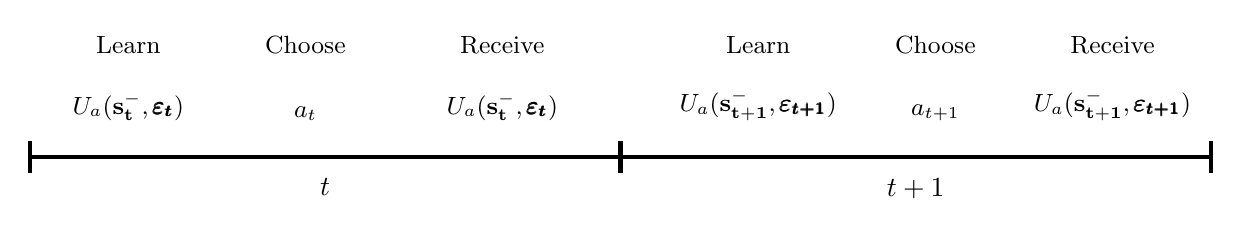
\begin{tikzpicture}
		\draw [ultra thick] (0,0) -- (15,0);
		\foreach \x in {0,7.5,15}
		\draw [ultra thick] (\x cm,0.2) -- (\x cm, -0.2);
		\small % derease fontsize
		\draw (1.25,0) node[above=0.35cm] {$U_a(\bold{s_t^-}, \pmb{\varepsilon_t})$};
		\draw (3.50,0) node[above=0.35cm] {$a_t$};
		\draw (6.0,0) node[above=0.35cm] {$U_a(\bold{s_t^-}, \pmb{\varepsilon_t})$};
		\draw (9.25,0) node[above=0.35cm] {$U_a(\bold{s_{t+1}^-}, \pmb{\varepsilon_{t+1}})$};
		\draw (11.5,0) node[above=0.35cm] {$a_{t+1}$};
		\draw (13.75,0) node[above=0.35cm] {$U_a(\bold{s_{t+1}^-}, \pmb{\varepsilon_{t+1}})$};
		
		\draw (1.25,0) node[above=1.2cm] {Learn};
		\draw (3.50,0) node[above=1.2cm] {Choose};
		\draw (6.0,0) node[above=1.2cm] {Receive};
		\draw (9.25,0) node[above=1.2cm] {Learn};
		\draw (11.5,0) node[above=1.2cm] {Choose};
		\draw (13.75,0) node[above=1.2cm] {Receive};
		
		\normalsize %reincrease fontsize
		\draw (3.75,0) node[below=0.15cm] {$t$};
		\draw (11.25,0) node[below=0.15cm] {$t+1$};
		%\draw (2.35,0) node[above=6pt, align=center] {(estimation \\ window]};
		\end{tikzpicture}
	\end{center}
\end{figure}

\noindent
At the beginning of each period $t$, the agent recognizes the reward shocks $\pmb{\varepsilon_{a,t}}$ (as opposed to the observer), and the shocks become part of the unobserved state space $\pmb{\varepsilon_t}$. Thus, the utilities $U_a(\bold{s_t^-}, \pmb{\varepsilon_t})$ are known to the agent in period $t$. However, he can only form expectations about rewards in the future as the alternative-specific shocks $\pmb{\varepsilon_{a,t}}$ are stochastic. The specification in \cite{Keane.1994} assumes the rewards shocks $\pmb{\varepsilon_{a,t}}$ to be serially uncorrelated. Therefore, prior shocks do not enter the state space. Next, the agent chooses his occupation $a_t$ based on the state space information. Then he receives the occupation-specific reward $U_a$. This flow repeats for each $t < T$.

Agents are rational and forward-looking. Future utilities are subject to time discount factor $\delta  \in [0,1]$. Hence, they choose their optimal sequence of occupations by maximizing the remaining expected, discounted life-time utility. This maximal value is given by the value function $V(\bold{s_t^-}, \pmb{\varepsilon_t})$.
\begin{align}
V(\bold{s_t^-}, \pmb{\varepsilon_t}) = \max_{\{a\}_{t=0}^T} \bigg\{ \sum_{t=0}^T \delta^t \int_{\pmb{\varepsilon_t}} U(\bold{s_{t}^{-}},\pmb{\varepsilon_{t}}, a_{t}) f(\pmb{\varepsilon_{t}})d^{|A|}\pmb{\varepsilon_{t}}\bigg\}
\end{align}
Value $V$ depends directly on time $t$ because $T$ is finite. Together with the discount factor $\delta$, this typically induces life-cycle behaviour. For example agents invest more in the earlier time periods and work (and consume) more in the following periods. As $\pmb{\varepsilon_{a,t}}$ are the only random parameters and serially independent, the expectation of $U(\bm{s_{t}^{-}},\pmb{\varepsilon_{t}}, a_{t})$ is given by the $|A|$-dimensional integral of U multiplied by the joint probability density function $f(\pmb{\varepsilon_{t}})$ with respect to $\pmb{\varepsilon_{t}}$. $|A|$ denotes the number of occupation choices.

Roughly sketched, the approach to solve the above maximization problem is given by the dynamic programming problem characterized by the Bellman equation (\cite{Bellman.1957}).\footnote{For more details, see \cite{Raabe.2019}, p. 9-19.}
\begin{align} \label{eq:Bellman}
V(\bold{s_t^-}, \pmb{\varepsilon_t}) = \max_{a_t} \bigg\{ U(\bold{s_t^-}, \pmb{\varepsilon_t}, a_t) + \delta \int_{\pmb{\varepsilon_t}} \max_{a_{t+1}} V_{a_{t+1}}(\bold{s_{t+1}^{-}},\pmb{\varepsilon_{t+1}}) f(\pmb{\varepsilon_{t+1}})d^{|A|}\pmb{\varepsilon_{t+1}}\bigg\}
\end{align}
\noindent
The Bellman equation states, that solving for the whole sequence of policy functions ${\{a^*\}_{t=0}^T}$ is equivalent to solving iteratively for each optimal, period-specific policy function $a_t^*(\bold{s_t^-}, \pmb{\varepsilon_t})$. For this purpose, choose $a_t$ for each period such that the current period utility and the discounted expected future lifetime utility (given the optimal choice of $a_{t+1}$) are maximized. The finite time horizon eases the problem as the value function for the last period $T$ simplifies to $V(\bold{s_T^-}, \pmb{\varepsilon_T}) = \max_{a_T} U(\bold{s_T^-}, \pmb{\varepsilon_T}, a_T)$. With this condition the problem can be solved for all states by iterating backwards. Given initial states and random draws for the  unobservable shocks $\pmb{\varepsilon_t}$ for each period, these policy equations are used to simulate the occupational paths for a number of agents.\\

\noindent
This paragraph addresses the alternative-specific utility functions $U_a(\bold{s_t^-}, \pmb{\varepsilon_t})$ which finally pins down the model in \cite{Keane.1994}. There are four different occupations, $b$, $w$, $e$ and $h$, of which occupations $b$ and $w$ are defined by the same type of utility function. In the following, I will explain how the first two utility functions roughly model characteristics for working in the blue and the white collar sector and how the latter two equations sketch receiving institutional education and staying at home. The utility functions for occupations $b$ and $w$, $U_b$ and $U_w$ equal the respective wage in USD, $W_{b,t}$ and $W_{w,t}$. It is assumed that there is a direct mapping from USD to utility. The wage equations are given by the Mincer equation for earnings (\cite{Mincer.1958}):
\begin{equation} \label{eq:returns_b_w}
\begin{aligned}
U_b(\bold{s_t^-}, \pmb{\varepsilon_t}) &= W_{b,t}^{-} = \text{exp}\big\{\beta^b + \beta_e^b x_{e,t} + \beta_b^b x_{b,t} + \beta_{bb}^b x^2_{b,t} + \beta_w^b x_{w,t} + \beta_{ww}^{b} x^2_{w,t} + \varepsilon_{b,t}\big\} \\
U_w(\bold{s_t^-},\pmb{\varepsilon_t}) &= W_{w,t}^{-} = \text{exp}\big\{\beta^w + \beta_e^w x_{e,t} + \beta_w^w x_{w,t} + \beta_{ww}^w x^2_{w,t} + \beta_b^w x_{b,t} + \beta_{bb}^{w} x^2_{b,t} + \varepsilon_{w,t}\big\}
\end{aligned}
\end{equation}
Both equations comprise of a constant term, years of schooling $x_{e,t}$, linear and quadratic terms of occupation experience, and cross-occupational experience and the  respective shocks in $\pmb{\varepsilon_t}$. $\pmb{\beta}$ is the vector of coefficients\footnote{The notation for $\pmb{\beta}$ includes two references: The superscript indicates the occupation-specific utility that "receives" the coefficients. The subscripts indicate the occupation-specific experience or abbreviates the condition that "sends" the coefficients. Thus, coefficients for constant terms do not have a subscript. Coefficients for quadratic terms are marked by twice the respective subscript.} that multiply factors that are called covariates by many structural economists.

The utilities for education, or schooling, and staying at home are given by the following functions. These functions are also called non-pecuniary rewards.
\begin{equation} \label{eq:returns_e_h}
\begin{aligned}
U_e(\bold{s_t^-}, \pmb{\varepsilon_t}) &= \beta^e + \beta_{col}^e \bold 1(x_{e,t} \geq 12) + \beta_{re}^e(1-\bold1(a_{t-1}=e)) + \varepsilon_{e,t} \\
U_h(\bold{s_t^-},\pmb{\varepsilon_t}) &= \beta^h + \varepsilon_{h,t} \\
\end{aligned}
\end{equation}
\noindent
$\beta^e$ is the consumption reward of schooling. Function $\bold 1(x_{e,t} \geq 12)$ indicates whether an agent has completed high school. $\beta_{col}^e$ is the post-secondary tuition cost of schooling and $\beta_{re}^e$ is an adjustment cost for returning to school when the agent chose another occupation the previous period ($a_{t-1}\neq e$). $\beta^h$ is the mean reward for staying at home.

It is assumed that $\pmb{\varepsilon_{a,t}}$ follows a joint normal distribution, such that $\pmb{\varepsilon_{a,t}} \sim \mathcal{N}(0,\,\pmb{\Sigma_\varepsilon})$. \pmb{$\Sigma_\varepsilon$} denotes the covariance matrix for the shocks $\pmb{\varepsilon_{a,t}}$. $\sigma_a^{2}$ and $\sigma^{2}_{a(j),a(k\neq j)}$ denote the alternative-specific variances and covariances in \pmb{$\Sigma_\varepsilon$}. Shocks are serially uncorrelated. Indices $j$ and $k$ are used to denote subsets of $a$.

Finally, there is a bijective mapping from time periods $t$ to age $16$ to $65$. The next subsection describes the estimation method.

\subsection{Simulated Maximum Likelihood Estimation}

The approach that \cite{Keane.1994} and this thesis use is the simulated maximum likelihood method (\cite{Albright.1977})\footnote{see \cite{Aguirregabiria.2010}, p. 42-44 and \cite{Raabe.2019}, p. 21-26 for a more detailed description}.

This method can be applied to a set of longitudinal data on occupational choices $a$ and, if available, wages $W_{a,t}^{-}$ of a sample of individuals $i \in I$ starting from age 16. To distinguish from the functions, let $\mathcal{W}^{-}_{a(k),t}$ denote the measured wages from this point on. For each period $t$, the recorded choices $a_0$, ..., $a_{t-1}$  imply the occupation-specific experiences $x_{a,t}$. Together with $t$, they constitute the observable state vector $\bold{s_t^-}$. Consequently, the measured, observable endogenous variables are $\bold{m}=(\bold{s_t^-},\mathcal{W}^{-}_{a,t})$. Given this setup, the goal is to estimate the exogenous model parameters $\pmb{\theta}=(\delta, \pmb{\beta}, \pmb{\Sigma_\varepsilon})$.\footnote{Improvements over \cite{Keane.1994} in this thesis' estimation are that, first, it is not assumed that the standard errors of the parameters estimates are uncorrelated, and second, that $\beta$ is not left out of the estimation.} Thus in the following, every probability is a function of the exogenous model parameters.
The approach for computation of the likelihood function $L_{\bold{m}}(\pmb{\theta})$ of the observables in the data begins with the individual latent variable representation in period $t$.
\begin{align}
a_t = \argmax_a V_a(\bold{s_t^-},\pmb{\varepsilon_t})
\end{align}
As $a_t$ and $\bold{s_t^-}$ is known, the next step is to derive the unobservable shocks $\pmb{\varepsilon_t}$ in terms of of both. Therefore, write the set of shock vectors for which the alternative-specific value function $V_{a(j)}$ is higher than the other value functions $V_{a(k\neq j)}$ in time $t$ as
\begin{align}
\pmb{\varepsilon_t}(a_t(j),\bold{s_t^-}) \defeq \{\pmb{\varepsilon_t}|V_{a_t(j)}(\bold{s_t^-},\pmb{\varepsilon_t}) = \max_a V_a(\bold{s_t^-},\pmb{\varepsilon_t})\}).
\end{align}
Note that the set condition is a function of the unobservable model parameters.

Consider first the case of non-working alternatives $a_t(j) \in [e,h]$. The probability of choosing $a_t(j)$ is the probability of set $\pmb{\varepsilon_t}(a_t(j),\bold{s_t^-})$. This probability equals the integral of the probability distribution function $f(\pmb{\varepsilon_t})$ over all elements of set $\pmb{\varepsilon_t}(a_t(j),\bold{s_t^-})$ with respect to $\pmb{\varepsilon_t}$. Formally,
\begin{align}
\text{p}\big(a_t(j) | \bold{s_t^-}\big) = \int_{\pmb{\varepsilon_t}(a_t(j),\bold{s_t^-})} f(\pmb{\varepsilon_t}) d^{|A|} \pmb{\varepsilon_t}.
\end{align}
\noindent
The second case is $a_t(k) \in [b,w]$. Assuming the dataset contains wages for the working alternatives $a_t(k)$, the probabilities of choosing $a_t(k)$ take a few steps more to compute. In the first step, note from the wage equations that the the alternative-specific shocks $\pmb{\varepsilon_{a,t}}$ are log normally distributed. Second, in contrary to the non-working alternatives, by using (\ref{eq:returns_b_w}), the shocks can directly be expressed as a function of the alternative-specific model parameters $\pmb{\beta_{a(k)}}$ by inserting the inferred alternative-specific experiences $\pmb{x_{a(k),t}}$ into $W_{a(k),t}$ and subtracting the expression from the observed wage $\mathcal{W}^{-}_{a(k),t}$ for one individual, where both wages are logarithmized. Thus,
\begin{align} \label{eq:epsilon}
\varepsilon_{a(k),t} = \text{ln}(\mathcal{W}^{-}_{a(k),t}) - \text{ln}(W_{a(k),t}^{-}).
\end{align}
Third, the alternative-specific shocks $\pmb{\varepsilon_{a,t}}$ are not distributed independently. Since $\varepsilon_{a(k),t}$ can be inferred from the
observed wage $\mathcal{W}^{-}_{a(k),t}$, the information can be used to form the expectation about the whole error distribution. Therefore, the probability of choosing occupation $a_t(k)$ conditional on observed states and wages writes

\noindent
\begin{align}
\text{p}\big(a_t(k) | \bold{s_t^-},W_{a(k),t}\big) = \int_{\pmb{\varepsilon_t}(a_t(k),\bold{s_t^-})} f(\pmb{\varepsilon_t}|\varepsilon_{a(k),t}) d^{|A|} \pmb{\varepsilon_t}.
\end{align}
Applying integration by substitution yields the following expression for the probability of the one observed wage:\footnote{See \cite{Raabe.2019}, p. 29 for more details}
\begin{align}
\text{p}\big(\mathcal{W}^{-}_{a(k),t} | \bold{s_t^-}\big) = \omega_t^{-1} \frac{1}{\sigma_{a(k)}} \phi\bigg(\frac{\varepsilon_{a(k),t}}{\sigma_{a(k)}}\bigg)
\end{align}
Here, $\omega_t^{-1}$ is the Jacobian of the transformation from observed wage $\mathcal{W}^{-}_{a(k),t}$ to error $\varepsilon_{a(k),t}$ in (\ref{eq:epsilon}) and $\phi$ is the standard normal probability density function.
Finally, the joint probability of observing choice $a_t(k)$ and wage $\mathcal{W}^{-}_{a(k),t}$ conditional on the observed states is given by the product of the two probabilities above:
\begin{align}
\text{p}\big(a_t(k),\mathcal{W}^{-}_{a(k),t}|\bold{s_t^-}\big) = \text{p}\big(a_t(k)|\bold{s_t^-}, \mathcal{W}^{-}_{a(k),t}\big)\text{p}\big(\mathcal{W}^{-}_{a(k),t}|\bold{s_t^-}\big)
\end{align}
Based on these results, the likelihood contribution of one individual $i$ can thus be written as the product of time-specific probabilities to observer the observable endogenous variables:
\begin{align}
L^{i}_{\bold{m}}(\pmb{\theta}) = P\big(\{a_{t,}^{i},\mathcal{W}^{-,i}_{a,t,}\}_{t=0}^T\big) = \prod_{t=0}^{T} \text{p}\big(a_t^{i},\mathcal{W}_{a,t}^{-,i}|\bold{s_t^{-,i}}\big)
\end{align}
Therefore, the sample likelihood is given by the product of the individual likelihoods over the whole sample of individuals:
\begin{align} \label{eq:sample-likelihood}
L_{\bold{m}}(\pmb{\theta}) = P\big(\big\{\{a_{t,}^{i},\mathcal{W}^{-,i}_{a,t,}\}_{t=0}^T\big\}_{i \in I}\big) = \prod_{i \in I}\prod_{t=0}^{T} \text{p}(a_t^{i},\mathcal{W}_{a,t}^{-,i}|\bold{s_t^{-,i})}
\end{align}
Since the probabilities are functions of the exogenous parameters $\pmb{\theta}$, the simulated maximum likelihood estimator $\pmb{\hat{\theta}}$ is the vector of exogenous parameters that maximizes (\ref{eq:sample-likelihood}). As maximum likelihoods estimates are asymptotically normal\footnote{This property is an advantage of this thesis' estimation approach. It facilitates the uncertainty quantification via Monte Carlo sampling because there is a simple closed form for the marginal probability density available.}, these results are taken as the mean vector for the input parameters in the uncertainty quantification.

The procedure to estimate the parameter vector $\pmb{\theta}$ using the above calculation of the likelihood is as follows: First, The optimization algorithm of choice proposes a parameter vector. Second, the model is solved via backward induction. Third, using the policy functions, the likelihood is computed. These steps are iterated until the optimizer has found the maximal likelihood. 
\\

Finally, the computation of the variance of the estimator is described.\footnote{see \cite{Verbeek.2012}, p. 184-186} It is used as covariance matrix in the UQ. The asymptotic covariance of maximum likelihood estimator equals the inverse of the information matrix: $\text{Var}(\theta)=\text{I}(\theta)^{-1}$. The Fisher information matrix $\text{I}(\pmb{\theta})$ is given by the variance of the scores with respect to the parameters. The scores $\text{s}(\pmb{\theta})$ are the first derivatives of the likelihood function. Formally, these relationships are given by
\begin{align} \label{eq:scores}
\text{s}(\pmb{\theta}) \defeq \frac{\partial L_{\bold{m}}({\pmb{\theta}})} {\partial \pmb{\theta}} = \sum_{i \in I} \frac{L_{\bold{m}}^{i}(\pmb{\theta})}{\partial \pmb{\theta}} \defeq \sum_{i \in I}\text{s}_i(\pmb{\theta})
\end{align}
Having multiple individual likelihood contributions, the scores are in the form of the  Jacobian matrix.
Using the property that the values of scores $\E[\text{s}(\theta)]$ are zero at the maximum likelihood estimates, the variance of the scores that is also equal to the Fisher information writes
\begin{align} \label{eq:info-matrix}
\text{I}(\pmb{\theta}) = \text{Var}(\text{s}(\pmb{\theta})) = \E[\text{s}(\pmb{\theta})\text{s}(\pmb{\theta})'].
\end{align}
The estimator\footnote{The computation of $\text{Cov}(\pmb{\theta})$ by using the Jacobian of the individual likelihood contributions is chosen over other approaches because, first, it yields no error in the inversion step of $I(\pmb{\theta})$ and, second, the results are reasonably close to the similar specification in \cite{Keane.1994}.} for the asymptotic variance of the maximum likelihood estimator is thus given by
\begin{align}
\hat{\text{Cov}_J} = \bigg( \frac{1}{N} \sum_{i \in I} \text{s}_i(\pmb{\hat{\theta}})\text{s}_i(\pmb{\hat{\theta}})' \bigg)^{-1}
\end{align}
The intuition behind the above expression is the following: Estimator $\pmb{\hat{\theta}}$ maximizes the sample likelihood. This is equivalent to the estimator setting the sample scores to zero. However, the individual likelihood may not be zero at the optimal parameter vector for the sample likelihood. This variation is captured by the variance of the individual scores evaluated at $\pmb{\hat{\theta}}$. The relations in (\ref{eq:scores}) and (\ref{eq:info-matrix}) then imply that the inverse of the variance of the individual scores is equivalent to the variance of the maximum likelihood estimator.
\subsection{Numerical Implementation}

Besides the commonly used python libraries, the thesis uses the packages \textit{\citetalias{Respy-Stenzel.2019}} and \textit{\citetalias{Estimagic-Stenzel.2019}} to compute the QoI and to estimate the distribution of the input parameters. All other programs can be found in the  \citetalias{Stenzel.2020}.\\

\noindent
As standard deviations $\sigma_{a}$ are restricted to positive numbers, drawing them from the estimated unrestricted joint normal distribution can lead to erroneous results. Therefore, covariance matrix $\pmb{\Sigma_\varepsilon}$ is written in terms of the lower triangular matrix $\pmb{\Sigma_\varepsilon^c}$ obtained from the Cholesky decomposition of $\pmb{\Sigma_\varepsilon}$. The contained Cholesky factors are unrestricted and denoted by $c_{i}$ and $c_{i,j}$. $i$ and $j$ are positional indices. Thus, estimates for the Cholesky parameters and their variation replace the estimates for the covariance matrix in the estimation of the input parameters' distribution.

\subsection{Estimation Results}
\cite{Keane.1994} simulate data on fictional parameter values to test the estimation method. They obtain good results. The authors estimate mean and standard deviations for their fictional parameter values. However, they do not estimate covariances. Since this restriction seems unrealistic, the thesis computes its own parameter estimation. Table 2 presents the obtained estimates for mean and standard deviation of the model parameters $\pmb{\theta}$. The correlation terms can be found in the \citetalias{Stenzel.2020}.
[Include notes on Lindas esitmation.]

 The mean estimates for $\pmb{\theta}$ have the following economic implications: Occupation two is more skill-intensive or, more formally, has higher returns to education and occupational experience than occupation one. Additionally, experience in occupation one is rewarded in occupation two but not vice versa. The $c$ parameters are the Cholesky factors of the lower triangular matrix $C$ obtained from a Cholesky decomposition of the covariance matrix of the error vector. In this model specification, matrix $C$ coincides with shocks covariance matrix $\Sigma$. Therefore, the error terms are uncorrelated, as well.

The estimates for \citeauthor{Keane.1994}' fictional parametrization in Table \ref{tab:params} are the moments used to describe the input parameter distribution for the uncertainty quantification. An estimation for real data is not part of this thesis but can be interesting for future research.

\begin{figure}[H]
	\caption{Correlation between estimates for important input parameters}
	\centering
	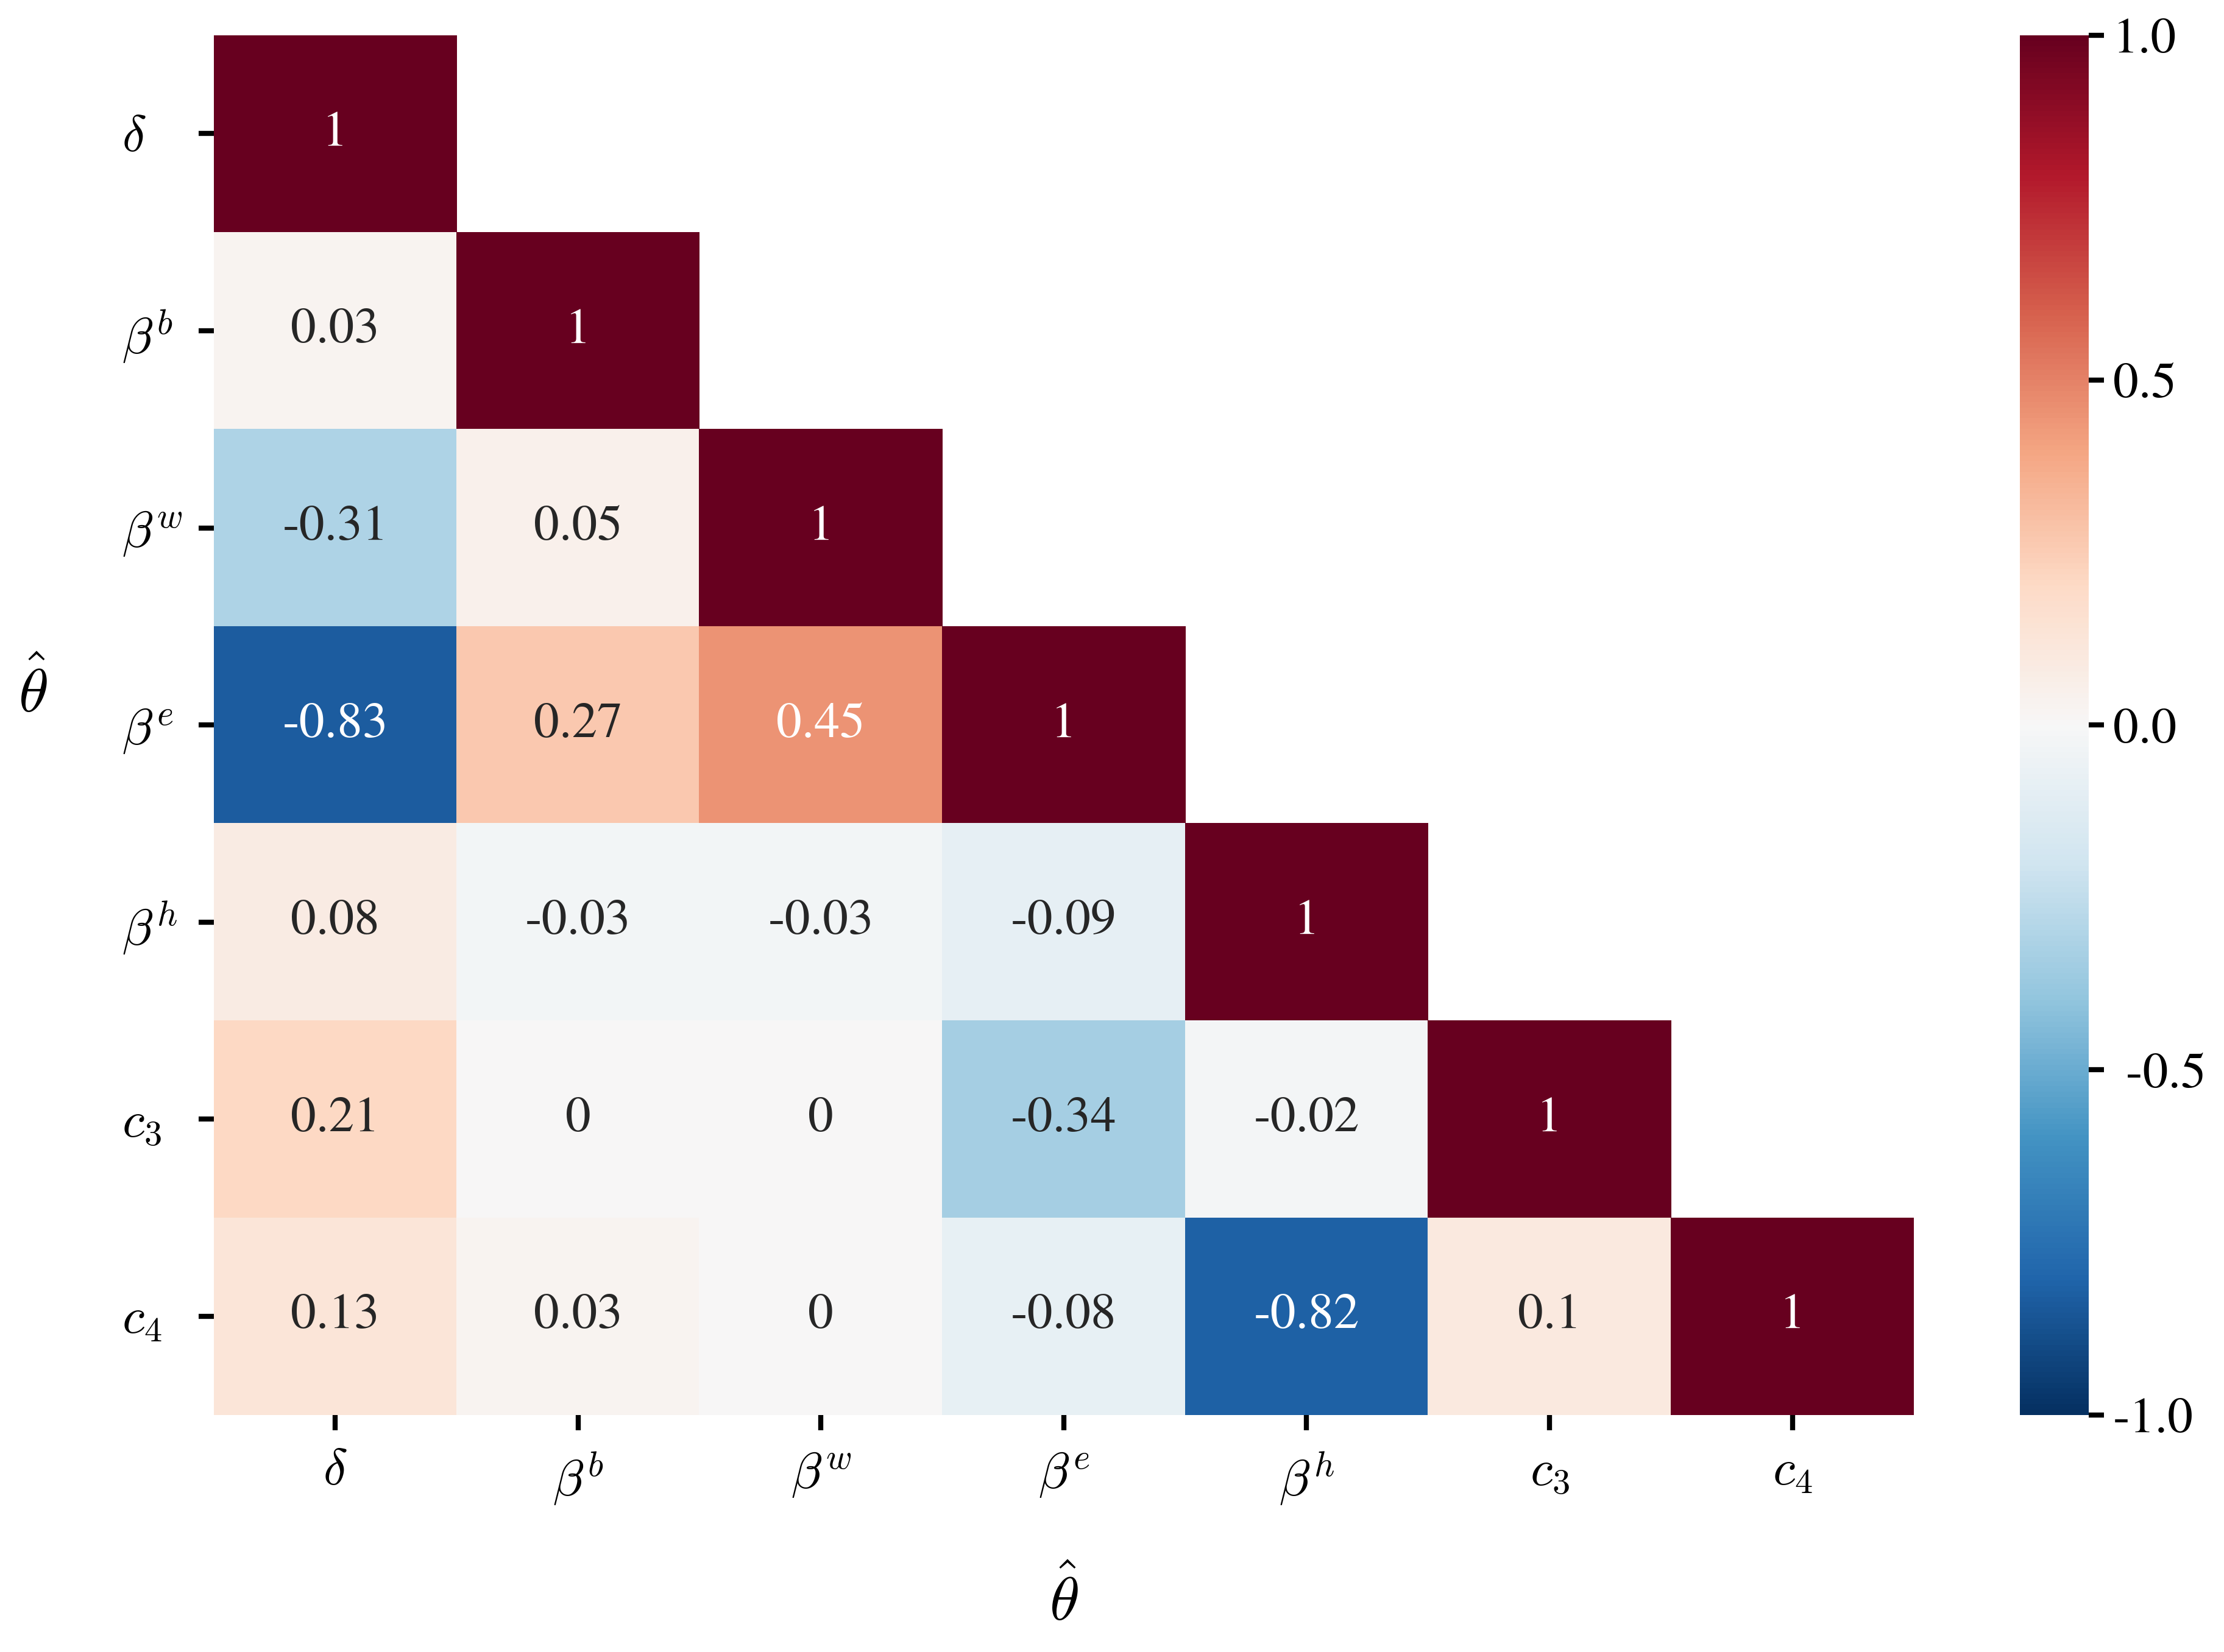
\includegraphics[scale=0.45]{../figures/heatmap_corr_chol}
\end{figure}

\subsection{Quantity of Interest}

The QoI for the uncertainty quantification is the effect of a \$500 college tuition subsidy on the average years of schooling. Formally, $\beta_{col}^{e,pol} 1(13 \leq s_a \leq 16) = \beta_{col}^e 1(13 \leq s_a \leq 16) - 500$. In \cite{Keane.1994}, the effect is an increase of 1.44 years (see Table 4, p. 668). The same figure computed with \citetalias{Respy-Stenzel.2019} is XX. [Include remarks on precision of KW94.] I choose this quantity because it is relevant to society in many respects, for example, education and inequality. Section XX expands this point. The QoI's relevance allows illustrating the importance of UQ in economics in the context of political decisions.

\begin{figure}[H]
	\caption{Comparison of occupation paths between scenarios}
	\centering
	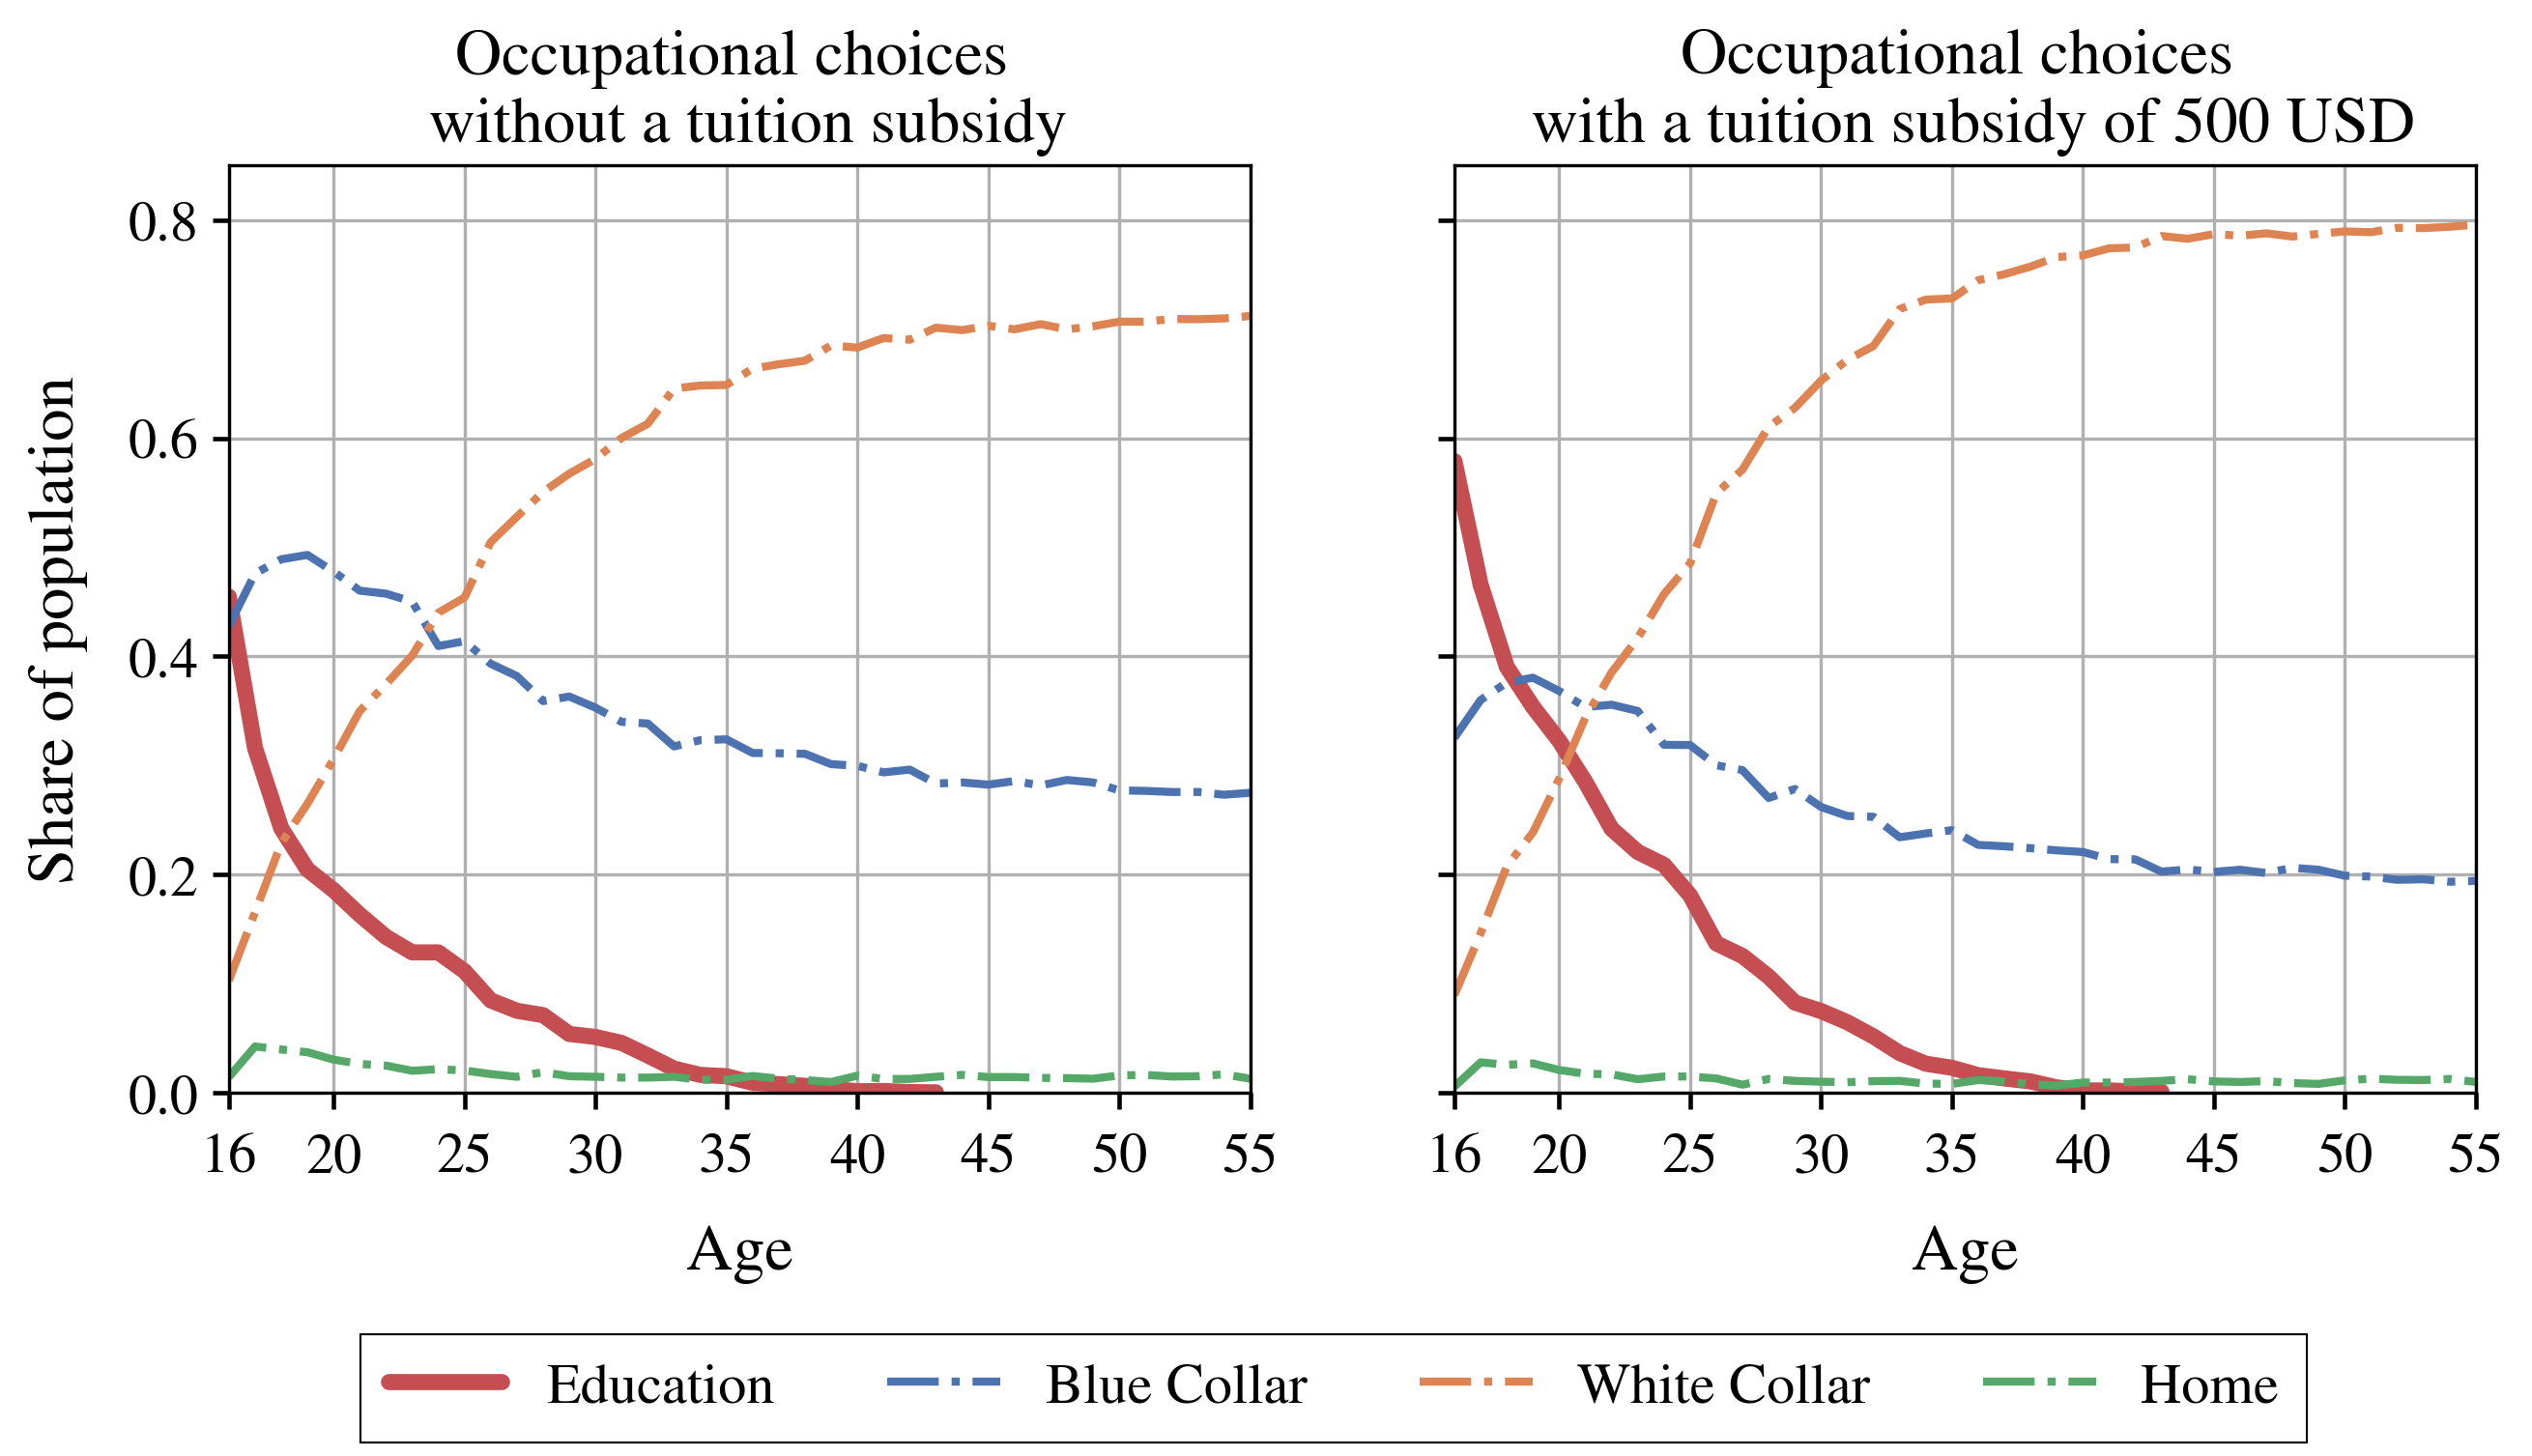
\includegraphics[scale=0.75]{../figures/occ_paths}
\end{figure}

% increase spacing between table columns
\setlength{\tabcolsep}{18pt} %from 6
\begin{table}[H] 
	\centering
	\begin{threeparttable}
		\caption[Model Parametrization]{Model Parametrization\tnote{a}}
		\label{tab:params}
		\renewcommand{\arraystretch}{1.2}%
		\begin{tabular}{cS[table-format=3.2]S[table-format=3.2]S[table-format=3.2]}
			\toprule
			{Parameter}     & {Mean\tnote{b}}   & {Estimated SD} & {SD in KW94} \\ \midrule
			\textit{General} \\
			$\delta$ & 0.95   & 0.00084 & \textit{-}	\\	\midrule
			\textit{Blue Collar}\\	
			$\beta^b$ & 9.21   & .013            & 0.014      \\
			$\beta_e^b$ & 0.038  &    0.0011        & 0.0015       \\
			$\beta_b^b$ & 0.033  & 0.00044            & 0.00079       \\
			$\beta_b^{bb}$ & -0.0005 & 0.000013           & 0.000019       \\
			$\beta_w^b$ & 0.0    & 0.00067             & 0.0024      \\
			$\beta_w^{bb}$ & 0.0    & 0.000029           & 0.000096       \\ \midrule
			\textit{White Collar}\\
			$\beta^w$ & 8.48   & 0.0076             & 0.0123      \\
			$\beta_e^w$ & 0.07   & 0.00047          & 0.00096       \\
			$\beta_w^w$ & 0.067  & 0.00055            & 0.0010      \\
			$\beta_w^{ww}$ & -0.001  & 0.000017           & 0.000030      \\
			$\beta_b^w$ & 0.022  & 0.00033           & 0.00090      \\
			$\beta_b^{ww}$ & -0.0005 & 0.000021         & 0.000070      \\ \midrule
			\textit{Education} \\
			$\beta^e$     & 0.0    & 329                & 459       \\
			$\beta_{col}^e$     & 0.0    & 156               & 410       \\
			$\beta_{re}^e$     & -4000   & 201                & 660       \\ \midrule
			\textit{Home} \\
			$\beta^h$    & 17750  & 388                & 1442      \\ \midrule
			\multicolumn{4}{l}{\textit{Standard Deviation/Correlation matrix}} \\
			$\sigma_{b}$      & 0.2    & 0.0015             & 0.0056      \\
			$\sigma_{w}$      & 0.25    & 0.0013             & 0.0046     \\
			$\sigma_{e}$      & 1500   & 108             & 350      \\
			$\sigma_{h}$      & 1500    & 173              & 786      \\
			$\rho_{b,w}$     & 0.0    & 0.026              & 0.023     \\
			$\rho_{b,e}$      & 0.0   & 0.096               & 0.412      \\
			$\rho_{w,e}$      & 0.0    & 0.077              &  0.379     \\
			$\rho_{b,h}$      & 0.0    & 0.16             &   0.911    \\
			$\rho_{w,h}$      & 0.0    & 0.087            & 0.624      \\
			$\rho_{e,h}$      & 0.0   & 0.12                & 0.870       \\ \bottomrule
		\end{tabular}
		\begin{tablenotes}
			\item[a] -
			\item[b] The mean estimates equal the true parameter values underlying the simulated sample up to an error of XX.

		\end{tablenotes}
	\end{threeparttable}
\end{table}
\section{Uncertainty Propagation}
\thispagestyle{plain} % surpress header on first page

\begin{figure}[H]
	\caption{Probability distribution of quantity of interest $q$}
	\centering
	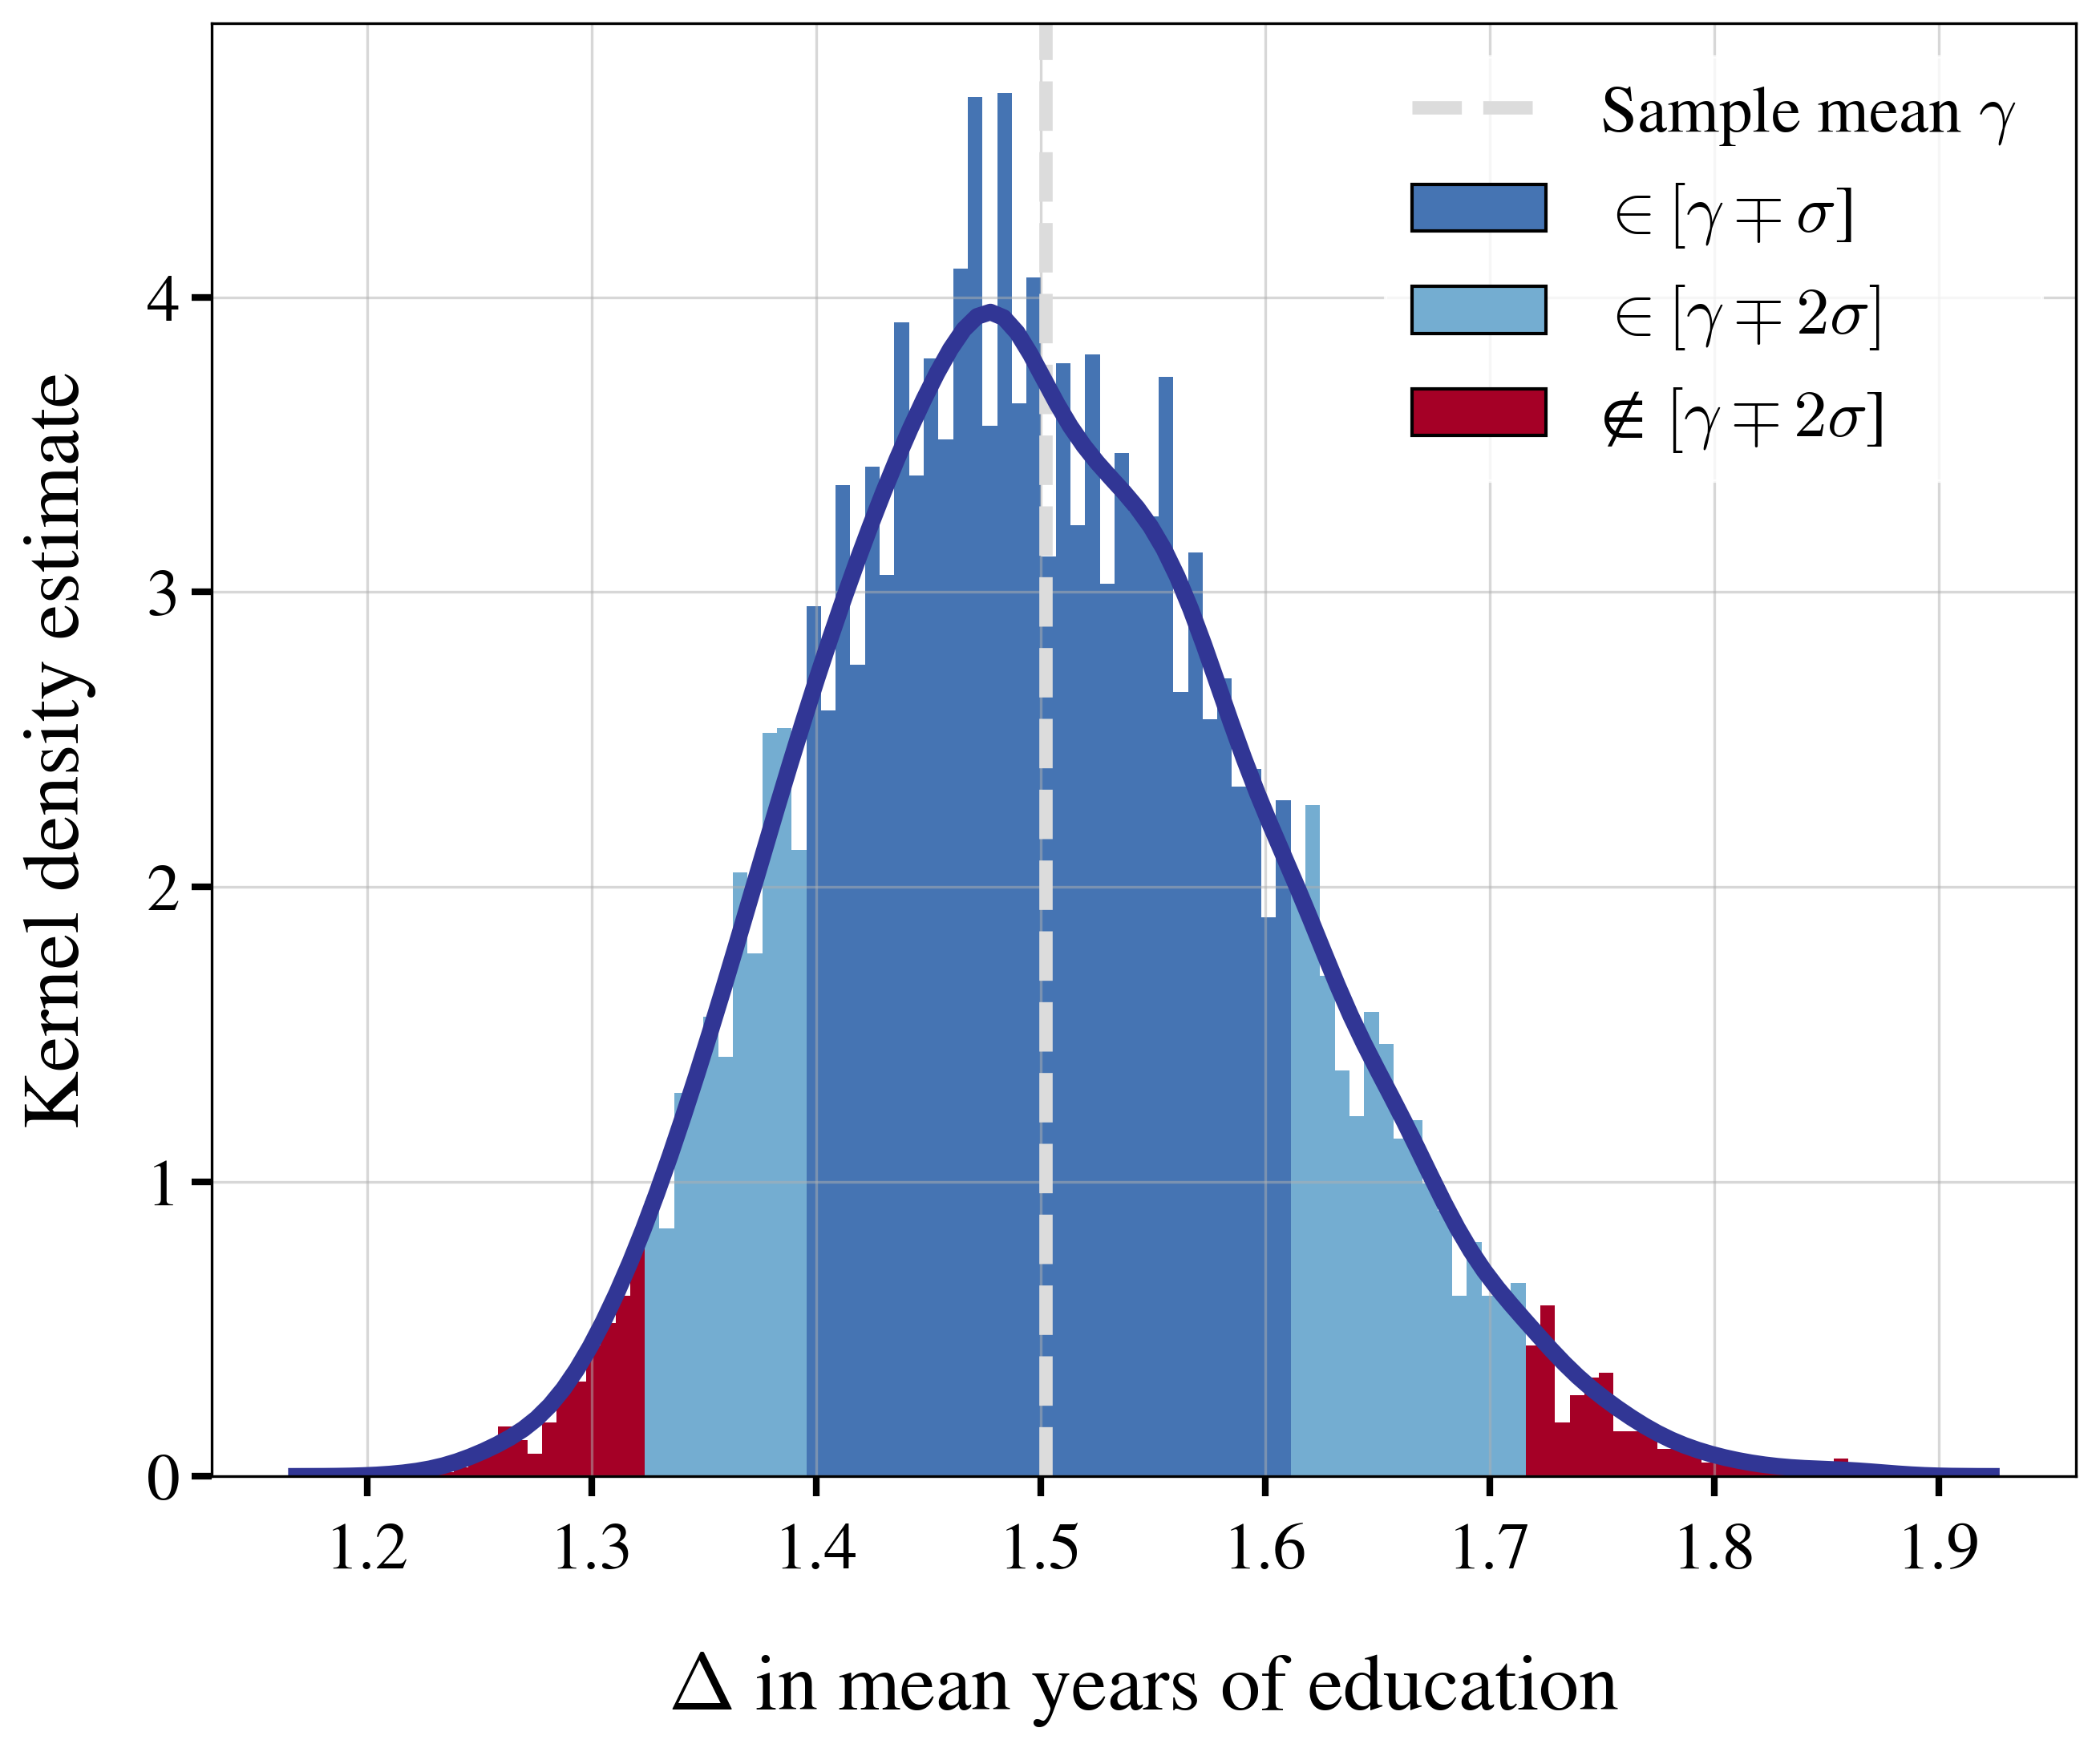
\includegraphics[scale=0.7]{../python/figures/distplot}
	\label{fig:dist}
\end{figure}




\section{Global Sensitivity Analysis}
\thispagestyle{plain} % surpress header on first page

[inlcude relative LOO error panel like in Miftakhova]


\subsection{Sobol' Indices}

\subsection{Univariate Effects}


[PCEs do not use Monte Carlo sampling, at least no converging one, i.e. a small number of evalations is enough]
\section{Discussion}
\thispagestyle{plain}  % surpress header on first page

This chapter discusses the UQ's findings, its value and implications. The first part deals with the more general results from the uncertainty analysis. Then, I address the qualitative GSA and identify important challenges for future research. This part of the discussion is organised along the areas measures, sampling and estimation.\\

\noindent
I analyse the uncertainty in  the effect of a 500 USD subsidy on annual tuition costs for higher education on the average years of education caused by the parametric uncertainty in the model of occupational choice by \cite{Keane.1994}. I find that the mean effect is an increase of 1.5 years in education for the whole population. {\color{red}Include many references that drive home the point how benefitial this is. Also note that e.g. heckman 2016 find that college graduation is not benefitial to everybody.}
I also find that the input uncertainty accounts for a standard deviation of 0.1 in the QoI. This is a relatively small level of variation. Abstracting from the model, these two basic results are important for economists in general. They do not help us to evaluate our model-based outcomes but they can also help us when we communicate with actors in the political arena. Indicating these results to, for example, important politicians and journalists proves a high level of sophistication and reflection. Therewith, our work may be received with higher regards and our work would be more impactful. Of course, the basis is that the economic results are relatively certain.\\

\noindent
The qualitative GSA includes three findings.
First, it confirms the conceptual analysis that the two EEs in \cite{ge2017extending} have two crucial disadvantages. The first is that the independent EE is not unaffected by the correlations between parameters. In fact, it deflates the impact of inputs according to their level of correlations with other parameters. As both parameters, the independent and the full EE have to be interpreted joint, one can not fix any parameter because this would require a reliable independent EE close to zero. The second drawback is that the draws in the numerator are in sample space and the draws in the denominator are in unit space. The analysis based on the redesigned EEs shows that it is not entirely clear which measure actually is adequate for factor fixing. However, the correlated and uncorrelated sigma-normalised mean absolute EEs, $\mu_\sigma^*$ are the only measures that are not detached from the scale of the QoI's standard deviation, $\sigma_Y$. This indicates that these measures are not only able to include the effect of the variation of $X_i$ on the level of $Y$ but also the effect on the variation of $Y$. I do not use this measure to recommend a fixing of any input parameter. The reason is that even for uncorrelated parameters, there is no consensus in the literature about what screening measures to choose, what cut-off criteria to use and what the particular links to the quantitative measures are. For example, \cite{campolongo2007effective} and \cite{ge2017extending} prefer the joint use of $\gamma^*$ and $\sigma$, \cite{kucherenko2009derivative} favour $(\frac{1}{r} \sum_{j=1}^{r} {d_i^2}^{(j)})/\pi^2 \sigma_Y$ and \cite{Smith.2014} highly recommends $\gamma^*_{\sigma}$.\\

\noindent
Second, the radial design generates higher EEs compared to the trajectory design for all parameters. In my view, the reason is that the radial design can generate steps $b-a$ as large as the whole sample space. This is a disadvantage for non-linear models with high variations. Furthermore, quantitative measures like the Sobol' indices do not consider such large differences. As these measures are variance-based, all draws are compared with the mean. This explanation is in line with the conceptual analysis in \cite{kucherenko2009derivative}. However, \cite{campolongo2007effective} find that the radial design is more precise in ranking the input parameters according to their effect on the variation in $Y$. Thus, it would be interesting to analyse these differences more closely. In any case, it is important to develop a sampling scheme that generates smaller steps $b-a$.\footnote{A possible path could be the following sketch for a hybrid design in unit space: the first row contains 0.5 for each column. Each step is a random draw in [0, 0.5]. Copy the changed draws to the next row as in the trajectory design and then shuffle each column to have equiprobable interactions for each parameter.}\\

\noindent
Third, the results indicate two potential interactions between maximum likelihood estimation and sensitivity analysis for correlated input parameters. The interactions require that the QoI is closely linked to the model observables $\pmb{\mathcal{D}}$.

Firstly, the correlated EE, $d_i^{c}$, is smaller than the uncorrelated EE, $d_i^{u}$, because parameters that have similar effects on observables $\pmb{\mathcal{D}}$ tend to be negatively correlated and those with opposite effects tend to be positively correlated. Therefore, the correlations "stabilise" the QoI against changes of specific input parameters.

Secondly, one observation from comparing the non-normalised measures to the sigma-normalised measures is that parameters that have a larger impact on the level of $Y$ tend to have a smaller impact on the variation in $Y$. This could be linked to a property of maximum likelihood estimation. The estimation implies larger standard errors for parameters with a smaller impact on the observables because they have a smaller influence on the probability of the observables. Consequently, a larger range of values for these less impactful parameters can potentially generate observables $\pmb{\mathcal{D}}$. Therefore, there might be an inverse relationship between ranking high with respect to measures that quantify the impact on the level of $Y$ and measures that deal with the variation in $Y$.

These arguments are rather speculative. It would be interesting if additional research could either confirm or contradict these hypotheses.

\section{Conclusion}
\thispagestyle{plain}  % surpress header on first page

\noindent
I analyse the uncertainty in the effect of a 500 USD subsidy on annual tuition costs for higher education on the average years of education caused by the parametric uncertainty in the model of occupational choice by \cite{Keane.1994}. The UQ has two stages. The first stage is an uncertainty analysis and the second stage is a quantitative GSA.\\

\noindent
The quantitative GSA finds that, first, the mean effect of the tuition subsidy is an increase of 1.5 years in education, and second, that the standard deviation is 0.1 years in education for the whole population. Therefore, the general parametric uncertainty is relatively small.\\

\noindent
The qualitative GSA and its conceptual preparation lead to three main results.
First, the sensitivity measures developed in \cite{ge2017extending} can not be used to rank input parameters according to their impact on the output variation because the independent EE is not unaffected by the correlations between input parameters.

The thesis develops two updated measures: The correlated and uncorrelated EEs, $d_i^{c}$ and $d_i^{u}$. The second finding is that the sigma-normalised mean absolute correlated and uncorrelated EEs, $\mu^{*,c}_{\sigma}$ and $\mu^{*,u}_{\sigma}$, appear to be valuable screening measures. Nonetheless, I do not provide recommendations to fix specific parameters because, first, cut-off criteria for the qualitative measures, and second, the link between these measures and quantitative GSA measures remain unclear for functions with correlated input parameters.


Third, the radial sampling scheme produces larger effects than the trajectory scheme for all input parameters. This suggests that the changes to the input parameters in both schemes are too large to capture the QoI's variation appropriately.

% Resources
\newpage
\thispagestyle{plain} % no header on first page
\addcontentsline{toc}{section}{References} %toc steht für table of contents


\bibliography{../bibliography/literature}

% Appendix
\newpage
\thispagestyle{plain} % no header on first page
\addcontentsline{toc}{section}{Appendix} 

\chead{\textit{\nouppercase{Appendix}}}

\thispagestyle{plain} % surpress header on first page

\subsection{Appendix A: Tables}
\thispagestyle{plain} % surpress header on first page

\phantom{This text will be invisible} 
\hspace{20cm}
\begin{table}[H]
	\centering
	\caption{Overview of UQ literature}
	\label{tab:lit}
	\renewcommand{\arraystretch}{1.2}%
	\begin{tabular}{lc}
		\toprule
		Content                      & Number of articles \\ \midrule
		$Topics$                       &                    \\
		\qquad Climate economics            & 8                  \\
		\qquad Macroeconomics               & 4                 \\ \midrule
		$Analyses$                     &                    \\
		\qquad Uncertainty analysis      & 8                  \\
		\qquad Globabl sensitivity analysis & 7                  \\
		\qquad Local sensitivity analysis   & 2                  \\ \midrule
		$Measures$                     &                    \\
		\qquad Sobol' indices               & 6                  \\
		\qquad Univariate effects           & 4                  \\
		\qquad Density-based measures & 2                  \\ \midrule
		$Methods$                      &                    \\
		\qquad Monte Carlo sampling         & 7                  \\
		\qquad Latin hypercube sampling         & 3                  \\
		\qquad Surrogate model              & 7                  \\
		\qquad Polynomial chaos expansions  & 2                  \\
		\qquad Intrusive methods            & 2                  \\ \midrule
		& 14                 \\ \bottomrule
	\end{tabular}
\end{table}
\noindent

% increase spacing between table columns
\setlength{\tabcolsep}{18pt} %from 6
\begin{table}[H] 
	\centering
	\begin{threeparttable}
		\caption[Model Parameters]{Estimates for the distribution of input parameters}
		\label{tab:params}
		\renewcommand{\arraystretch}{1.2}%
		\begin{tabular}{cS[table-format=3.2]S[table-format=3.2]S[table-format=3.2]}
			\toprule
			{Parameter}     & {Mean}   & {Standard error (SE)} & {SE in KW94} \\ \midrule
			\textit{General} \\
			$\delta$ & 0.95   & 0.00084 & \textit{-}    \\    \midrule
			\textit{Blue-collar}\\    
			$\beta^b$ & 9.21   & .013            & 0.014      \\
			$\beta_e^b$ & 0.038  &    0.0011        & 0.0015       \\
			$\beta^b_b$ & 0.033  & 0.00044            & 0.00079       \\
			$\beta^b_{bb}$ & -0.0005 & 0.000013           & 0.000019       \\
			$\beta^b_w$ & 0.0    & 0.00067             & 0.0024      \\
			$\beta^b_{ww}$ & 0.0    & 0.000029           & 0.000096       \\ \midrule
			\textit{White-collar}\\
			$\beta^w$ & 8.48   & 0.0076             & 0.0123      \\
			$\beta^w_e$ & 0.07   & 0.00047          & 0.00096       \\
			$\beta^w_w$ & 0.067  & 0.00055            & 0.00090      \\
			$\beta^w_{ww}$ & -0.001  & 0.000017           & 0.000070     \\
			$\beta^w_b$ & 0.022  & 0.00033           & 0.0010      \\
			$\beta^w_{bb}$ & -0.0005 & 0.000021         & 0.000030      \\ \midrule
			\textit{Education} \\
			$\beta^e$     & 0.0    & 330                & 459       \\
			$\beta_{he}^e$     & 0.0    & 155               & 410       \\
			$\beta_{re}^e$     & -4000   & 202                & 660       \\ \midrule
			\textit{Home} \\
			$\beta^h$    & 17750  & 390                & 1442      \\ \midrule
			\multicolumn{4}{l}{\textit{Lower Triangular Cholesky Matrix}} \\
			$c_{1}$      & 0.2    & 0.0015             & 0.0056      \\
			$c_{2}$      & 0.25    & 0.0013             & 0.0046     \\
			$c_{3}$      & 1500   & 108             & 350      \\
			$c_{4}$      & 1500    & 176              & 786      \\
			$c_{1,2}$     & 0.0    & 0.0064              & 0.023     \\
			$c_{1,3}$      & 0.0   & 145               & 0.412      \\
			$c_{2,3}$      & 0.0    & 116             &  0.379     \\
			$c_{1,4}$      & 0.0    & 235             &   0.911    \\
			$c_{2,4}$      & 0.0    & 131            & 0.624      \\
			$c_{3,4}$      & 0.0   & 178                & 0.870       \\ \bottomrule
		\end{tabular}
	\end{threeparttable}
\end{table}

% Please add the following required packages to your document preamble:
% \usepackage{booktabs}
\setlength{\tabcolsep}{12pt} %from 6
\begin{table}[H]
	\centering
	\caption{Replication and Validation - trajectory design}
	\label{tab:repval1}
	\renewcommand{\arraystretch}{1.2}%
	\begin{threeparttable}
		\begin{tabular}{cS[table-format=3.2]S[table-format=3.2]S[table-format=3.2]S[table-format=3.2]}
			\toprule
			{Measure}     & {GM'17}   & {Repl. $\mu^{*}$}\tnote{$\dagger$} & {Repl. $\sigma$}\tnote{$\ddagger$} & {S'20} \\ \midrule
			
			
			& 1.20  & 1.36         & 0.83         & 1.00 \\
			\qquad $\mu^{*,ind}$                               & 1.30  & 1.48         & 0.91         & 1.00 \\
			& 3.20  & 3.11         & 1.94         & 1.00 \\
			&&&& \\
			& 0.55  & 0.00         & 0.56         & 0.00 \\
			\qquad $\sigma^{ind}$                            & 0.60  & 0.00         & 0.62         & 0.00 \\
			& 1.30  & 0.00         & 1.32         & 0.00 \\
			&&&& \\
			& 14.90 & 16.20        & 9.97         & 2.30 \\
			\qquad $\mu^{*,full}$                              & 12.50 & 13.45        & 8.31         & 1.91 \\
			& 10.00 & 9.93         & 6.18         & 1.41 \\
			&&&& \\
			& 6.50  & 0.00         & 6.74         & 0.00 \\
			\qquad $\sigma^{full}$                           & 5.50  & 0.00         & 5.63         & 0.00 \\
			& 4.00  & 0.00         & 4.20         & 0.00 \\		
			\bottomrule	
		\end{tabular}
		\begin{tablenotes}
			
			\item[$\dagger$] \footnotesize $0^{num}=0.00001$ and $l=4$. 
			\item[$\ddagger$] $0^{num}=0.00000001$ and $l=24$.\par
			
		\end{tablenotes}
	\end{threeparttable}
\end{table}

\phantom{This text will be invisible} 
\hspace{5cm} %linebreak.
% Please add the following required packages to your document preamble:
% \usepackage{booktabs}
\setlength{\tabcolsep}{12pt} %from 6
\begin{table}[H]
	\centering
	\caption{Replication and Validation - radial design}
	\label{tab:repval2}
	\renewcommand{\arraystretch}{1.2}%
	\begin{tabular}{cS[table-format=3.2]S[table-format=3.2]S[table-format=3.2]}
		\toprule
		{Measure}     & {GM'17}   & {Replication}  & {S'20} \\ 
		\midrule
		
		& 0.60  & 0.57         &  1.00 \\
		\qquad $\mu^{*,ind}$                               & 0.75  & 0.85         &  1.00 \\
		& 1.50  & 1.31         &  1.00 \\
		&&& \\
		& 0.20   & 0.10         &  0.00 \\
		\qquad $\sigma^{ind}$                            & 0.30   & 0.41         &  0.00 \\
		& 0.85  & 0.22         & 0.00 \\
		&&& \\
		& 7.50  & 6.84         &  2.30 \\
		\qquad $\mu^{*,full}$                              & 6.80   & 7.77         &  1.91 \\
		& 4.75  & 4.19         &  1.41 \\
		&&& \\
		& 2.90  & 1.15         &  0.00 \\
		\qquad $\sigma^{full}$                           & 2.65  & 3.68         &  0.00 \\
		& 2.50   & 0.70         &  0.00 \\ \bottomrule
	\end{tabular}
\end{table}

\newpage
\phantom{This text will be invisible} 
\vspace{10mm} %5mm vertical space
% Please add the following required packages to your document preamble:
% \usepackage{booktabs}
\begin{table}[H]
	\centering
	\caption{Comparison of sensitivity measures for a linear function}
	\label{tab:bad-mu}
	\begin{tabular}{@{}lccc@{}}
		\toprule
		Parameters & $S_i^T$ & $\gamma_i^*$ & $(\mu_i^* \frac{\sigma_{X_i}}{\sigma_Y})^2$ \\ \midrule
		$X_1$ & $9$                       & $3$   & $9$   \\
		$X_2$ & $8$                       & $2$   & $8$   \\
		$X_3$ & $9$                       & $1$   & $9$   \\ \bottomrule
	\end{tabular}
\end{table}

\newpage
\setlength{\tabcolsep}{22pt} %from 6
\begin{table}[H] 
	\centering
	\begin{threeparttable}
		\caption[Quantitative GSA measures by \cite{ge2017extending}]{EE-based measures by \cite{ge2017extending} for 100 trajectories}
		\label{tab:kw94gm17}
		\renewcommand{\arraystretch}{1.2}%
		\begin{tabular}{cS[table-format=3.2]S[table-format=3.2]@{\hskip 0.7in}|@{\hskip 0.5in}S[table-format=3.2]S[table-format=3.2]}
			
			{Parameter}     & {$\mu^{*,full}_T$}   & {$\mu^{*,ind}_T$} & {$\sigma^{*,full}_T$} & {$\sigma^{*,ind}_T$}\\ \midrule
			\textit{General} \\
			$\delta$ & 53.40   & 0.00 & 69.23 & 0.09   \\    \midrule
			\textit{Blue-collar}\\    
			$\beta^b$ & 3.55   & 0.05            & 4.38 & 0.07    \\
			$\beta_e^b$ & 39.84  &    0.05        & 49.69  & 0.07    \\
			$\beta^b_b$ & 77.21  & 0.05            & 90.23  & 0.07    \\
			$\beta^b_{bb}$ & 2616.50 & 0.05           & 3357.92  & 0.06     \\
			$\beta^b_w$ & 94.74    & 0.05             & 113.49  &  0.06  \\
			$\beta^b_{ww}$ & 1136.58    & 0.03          & 1405.94 &  0.04    \\ \midrule
			\textit{White-collar}\\
			$\beta^w$ & 5.07   & 0.05            & 6.42 &  0.06   \\
			$\beta^w_e$ & 90.25   & 0.07          & 111.50 &  0.08    \\
			$\beta^w_w$ & 82.88  & 0.05            & 103.66 &  0.07   \\
			$\beta^w_{ww}$ & 2444.13  & 0.06           & 3044.69 & 0.07   \\
			$\beta^w_b$ & 452.91 & 0.07           & 490.31 &  0.09   \\
			$\beta^w_{bb}$ & 4317.58 & 0.05         & 4851.54 &  0.06   \\ \midrule
			\textit{Education} \\
			$\beta^e$     & 0.00    & 0.09             & 0.00&  0.10   \\
			$\beta_{he}^e$     & 0.00    & 0.11              & 0.00  & 0.13    \\
			$\beta_{re}^e$     & 0.00  & 0.04               & 0.000  &   0.09  \\ \midrule
			\textit{Home} \\
			$\beta^h$    & 0.00  & 0.04                 & 0.00  & 0.05     \\ \midrule
			\multicolumn{4}{l}{\textit{Lower Triangular Cholesky Matrix}} \\
			$c_{1}$      & 27.94    & 0.07             & 33.72 &  0.08   \\
			$c_{2}$      & 31.89   & 0.05             & 38.58 & 0.06   \\
			$c_{3}$      & 0.00   & 0.06             & 0.00 & 0.07    \\
			$c_{4}$      & 0.00    & 0.04              & 0.00 & 0.09    \\
			$c_{1,2}$     & 12.41   & 0.06            & 14.33 &  0.08  \\
			$c_{1,3}$      & 0.00   & 0.09              & 0.00 &  0.10   \\
			$c_{2,3}$      & 0.00    & 0.05             &  0.00 &   0.06 \\
			$c_{1,4}$      & 0.00    & 0.04            &   0.00 &  0.05 \\
			$c_{2,4}$      & 0.00    & 0.03           & 0.00  &  0.03  \\
			$c_{3,4}$      & 0.00   & 0.04                & 0.00  &  0.05   \\ \bottomrule
		\end{tabular}
	\end{threeparttable}
\end{table}


\newpage
\setlength{\tabcolsep}{22pt} %from 6
\begin{table}[H] 
	\centering
	\begin{threeparttable}
		\captionsetup{format=hang}
		\caption[Quantitative GSA measures for the Occupational Choice Model]{Mean absolute correlated and uncorrelated elementary effects. The results are computed from 100 subsamples in trajectory and radial design.}
		\label{tab:devees}
		\renewcommand{\arraystretch}{1.2}%
		\begin{tabular}{cS[table-format=3.2]S[table-format=3.2]@{\hskip 0.7in}|@{\hskip 0.5in}S[table-format=3.2]S[table-format=3.2]}
			
			{Parameter}     & {$\mu^{*,c}_T$}   & {$\mu^{*,c}_R$} & {$\mu^{*,u}_T$} & {$\mu^{*,u}_R$}\\ \midrule
			\textit{General} \\
			$\delta$ & 17   & 23 & 476 & 415   \\    \midrule
			\textit{Blue-collar}\\    
			$\beta^b$ & 1   & 3            & 43 & 88    \\
			$\beta_e^b$ & 11  &    14        & 406  & 443    \\
			$\beta^b_b$ & 25  & 51            & 688  & 1169    \\
			$\beta^b_{bb}$ & 871 & 934           & 15540  & 17860     \\
			$\beta^b_w$ & 29    & 48             & 73  &  143  \\
			$\beta^b_{ww}$ & 389    & 460           & 869 &  1183    \\ \midrule
			\textit{White-collar}\\
			$\beta^w$ & 1   & 3            & 50 &  117   \\
			$\beta^w_e$ & 26   & 28          & 943 &  852    \\
			$\beta^w_w$ & 24  & 47            & 718 &  1521   \\
			$\beta^w_{ww}$ & 933  & 997           & 12257 & 18069   \\
			$\beta^w_b$ & 131 & 127           & 309 &  356   \\
			$\beta^w_{bb}$ & 1230 & 1352         & 2088 &  2477   \\ \midrule
			\textit{Education} \\
			$\beta^e$     & 0.0008    & 0.0002              & 0.001&  0.003   \\
			$\beta_{he}^e$     & 0.0001    & 0.0002              & 0.001  & 0.001    \\
			$\beta_{re}^e$     & 0.0003   & 0.0002               & 0.0003  &   0.0006  \\ \midrule
			\textit{Home} \\
			$\beta^h$    & 0.0003  & 0.0003                 & 0.00002  & 0.00002     \\ \midrule
			\multicolumn{4}{l}{\textit{Lower Triangular Cholesky Matrix}} \\
			$c_{1}$      & 8    & 16             & 18 &  37   \\
			$c_{2}$      & 8   & 11             & 22 & 24   \\
			$c_{3}$      & 0.0004   & 0.0004             & 0.0004 & 0.0007    \\
			$c_{4}$      & 0.0004    & 0.00008              & 0.0002 & 0.0003    \\
			$c_{1,2}$     & 4   & 4            & 10 &  10  \\
			$c_{1,3}$      & 0.0005   & 0.0006              & 0.0006 &  0.0005   \\
			$c_{2,3}$      & 0.0003    & 0.0005             &  0.0006 &   0.001 \\
			$c_{1,4}$      & 0.00004    & 0.00005            &   0.0004 &  0.0005 \\
			$c_{2,4}$      & 0.0001    & 0.0002           & 0.0001  &  0.0002  \\
			$c_{3,4}$      & 0.0001   & 0.0001                & 0.00008  &  0.0001   \\ \bottomrule
		\end{tabular}
	\end{threeparttable}
\end{table}


\subsection{Appendix B: Figures}
\thispagestyle{plain} % surpress header on first page

\vspace{10mm} %5mm vertical space
\begin{figure}[H]
	\caption{Timeline of events} \label{fig:order}
	\vspace{-0.0cm}
	
	\begin{center}        
		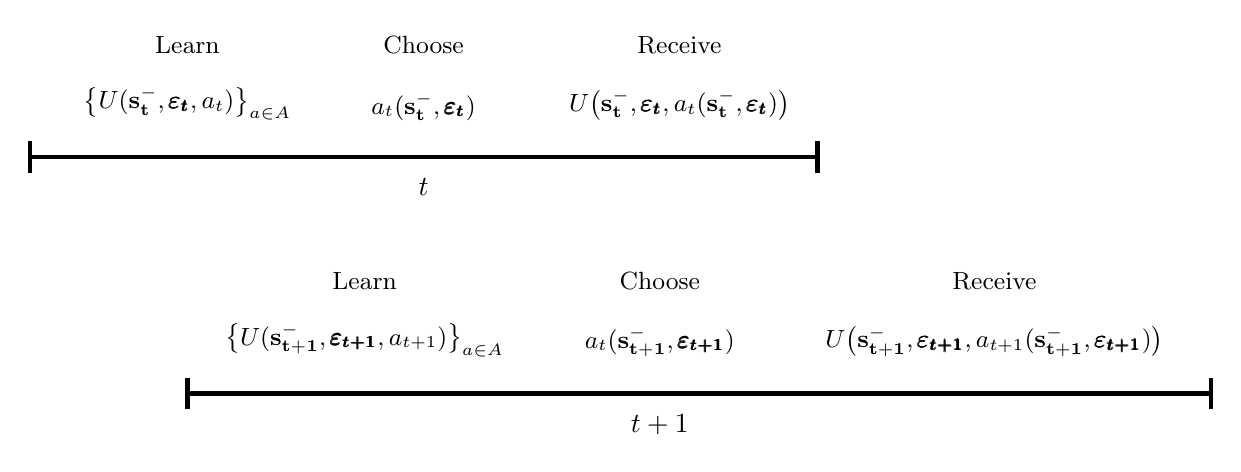
\begin{tikzpicture}
		% upper part
		\draw [ultra thick] (0,0) -- (10,0);
		\foreach \x in {0,10}
		\draw [ultra thick] (\x cm,0.2) -- (\x cm, -0.2);
		\small % derease fontsize
		\draw (2.0,0) node[above=0.35cm] {$\big\{U(\bold{s_t^-}, \pmb{\varepsilon_t},a_t)\big\}_{a \in A}$};
		\draw (5.0,0) node[above=0.35cm] {$a_t(\bold{s_t^-}, \pmb{\varepsilon_t})$};
		\draw (8.25,0) node[above=0.35cm] {$U\big(\bold{s_t^-}, \pmb{\varepsilon_t},a_t(\bold{s_t^-}, \pmb{\varepsilon_t})\big)$};
		
		\draw (2.0,0) node[above=1.2cm] {Learn};
		\draw (5.0,0) node[above=1.2cm] {Choose};
		\draw (8.25,0) node[above=1.2cm] {Receive};
		
		\normalsize %reincrease fontsize
		\draw (5.0,0) node[below=0.15cm] {$t$};
		
		%lower part
		\draw [ultra thick] (2.0,-3) -- (15,-3);
		\foreach \x in {2.0,15}
		\draw [ultra thick] (\x cm,-2.8) -- (\x cm, -3.2);
		\small % derease fontsize
		\draw (4.25,-3) node[above=0.35cm] {$\big\{U(\bold{s_{t+1}^-}, \pmb{\varepsilon_{t+1}},a_{t+1})\big\}_{a \in A}$};
		\draw (8.0,-3) node[above=0.35cm] {$a_t(\bold{s_{t+1}^-}, \pmb{\varepsilon_{t+1}})$};
		\draw (12.25,-3) node[above=0.35cm] {$U\big(\bold{s_{t+1}^-}, \pmb{\varepsilon_{t+1}},a_{t+1}(\bold{s_{t+1}^-}, \pmb{\varepsilon_{t+1}})\big)$};
		
		\draw (4.25,-3) node[above=1.2cm] {Learn};
		\draw (8.0,-3) node[above=1.2cm] {Choose};
		\draw (12.25,-3) node[above=1.2cm] {Receive};
		
		\normalsize %reincrease fontsize
		\draw (8.0,-3) node[below=0.15cm] {$t+1$};      
		
		%\draw (2.35,0) node[above=6pt, align=center] {(estimation \\ window]};
		\end{tikzpicture}
	\end{center}
\end{figure}

\vspace{20mm} %5mm vertical space


\begin{figure}[H]
	\caption{Correlations between estimates for important input parameters}
	\centering
	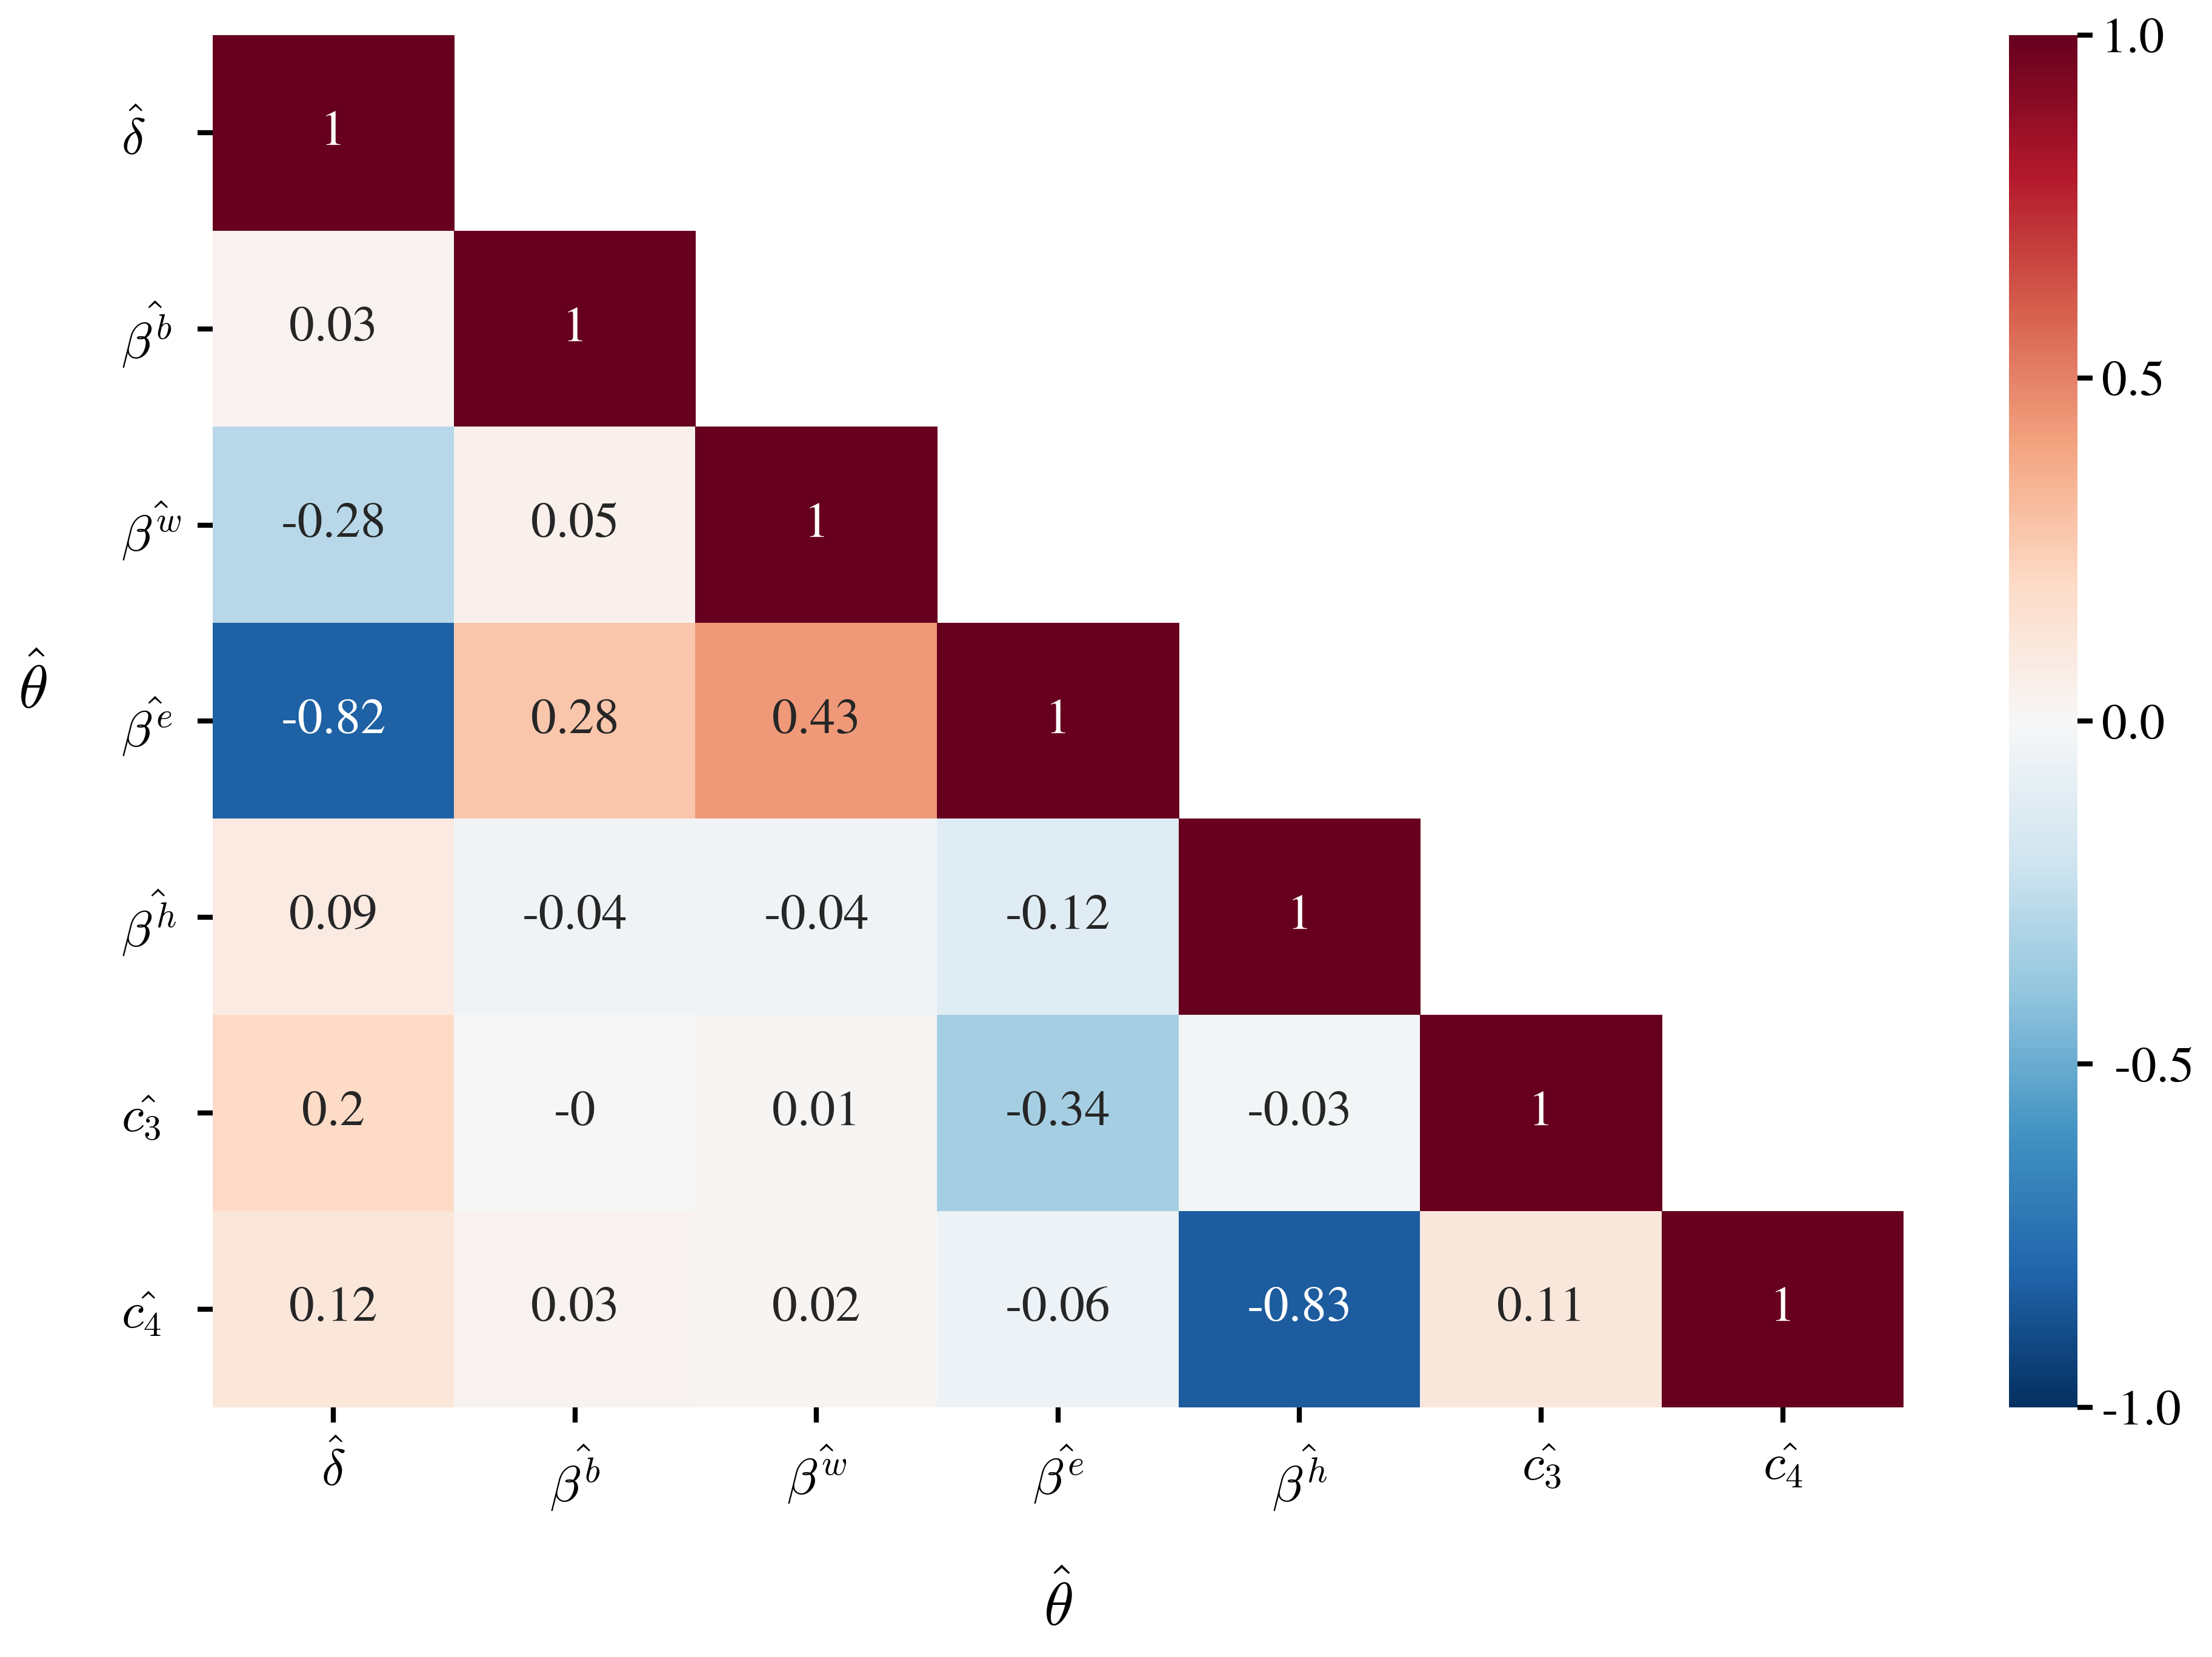
\includegraphics[scale=0.45]{../scrypy/figures/heatmap}
	\label{fig:corr}
\end{figure}
\newpage
\phantom{This text will be invisible} 
\vspace{20mm} %5mm vertical space
\begin{figure}[H]
	\caption[Comparison of shares of occupation decisions]{Comparison of shares of occupation decisions over time between scenarios}
	\centering
	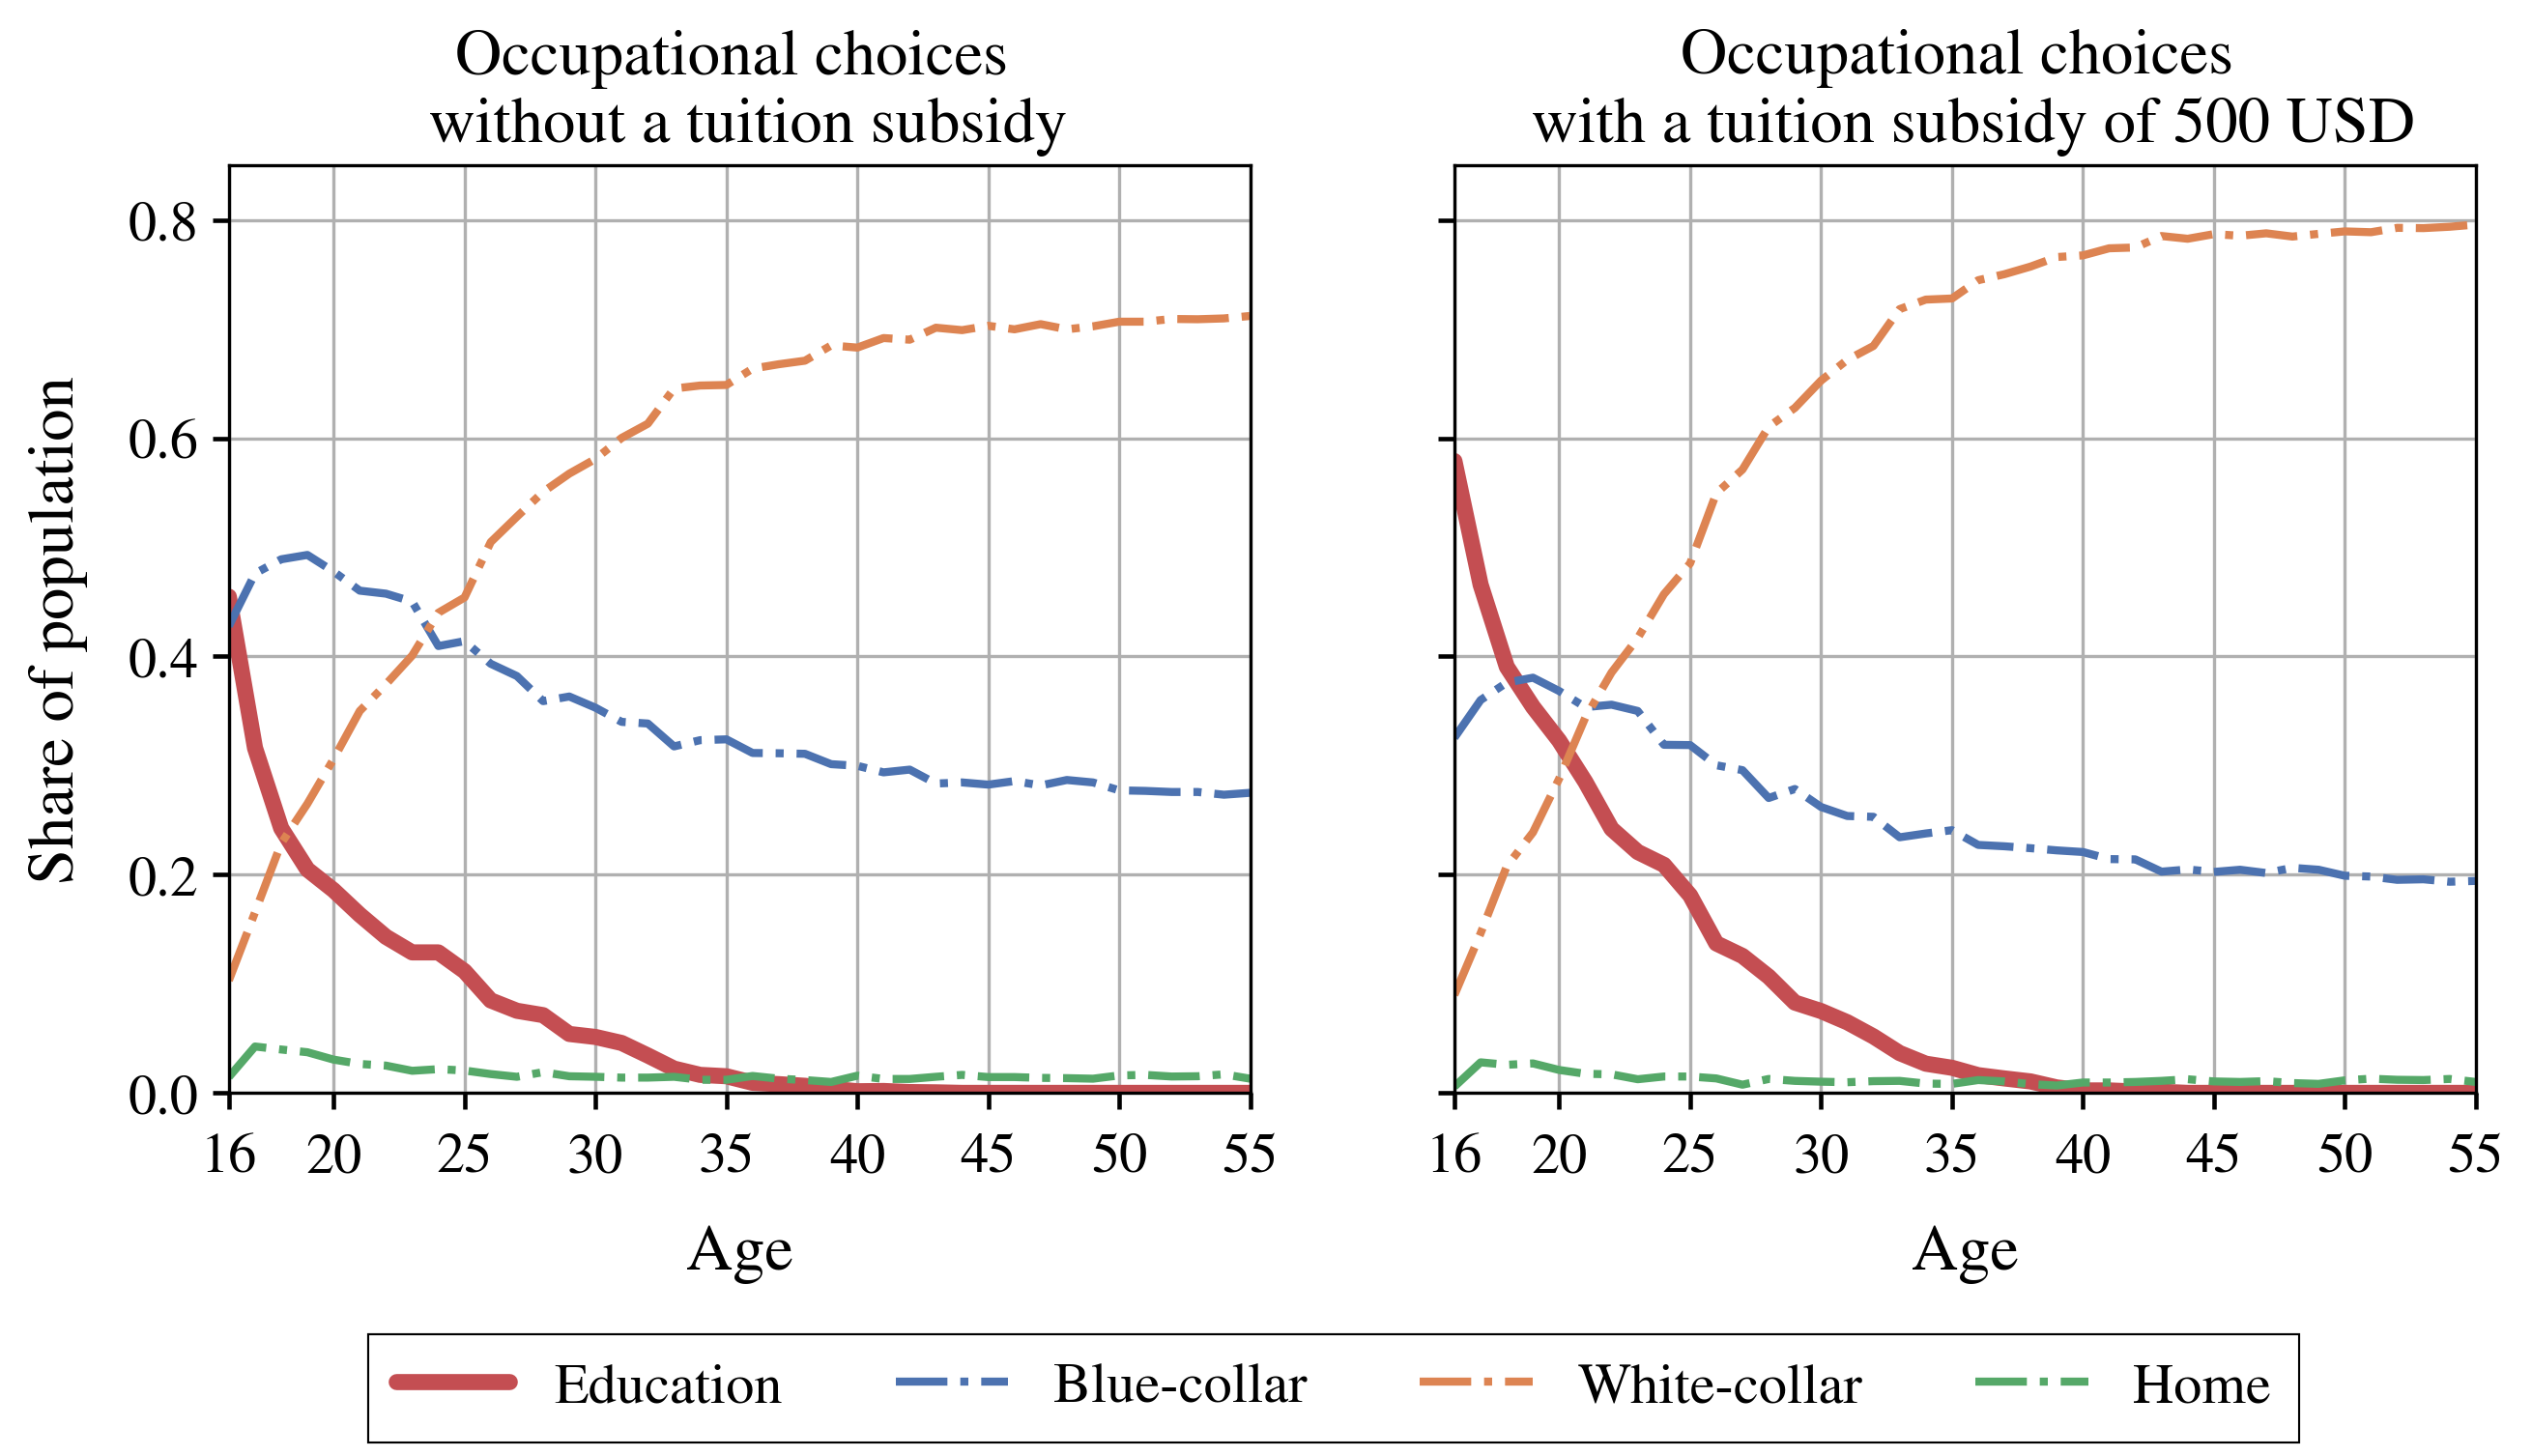
\includegraphics[scale=0.75]{../scrypy/figures/occ_choice_shares}
	\label{fig:paths}
\end{figure}

\vspace{10mm} %5mm vertical space

\begin{figure}[H]
	\caption[Grid points in standard normal sample]{Grid points in standard normal sample space for trajectory design with $l=4$}
	\centering
	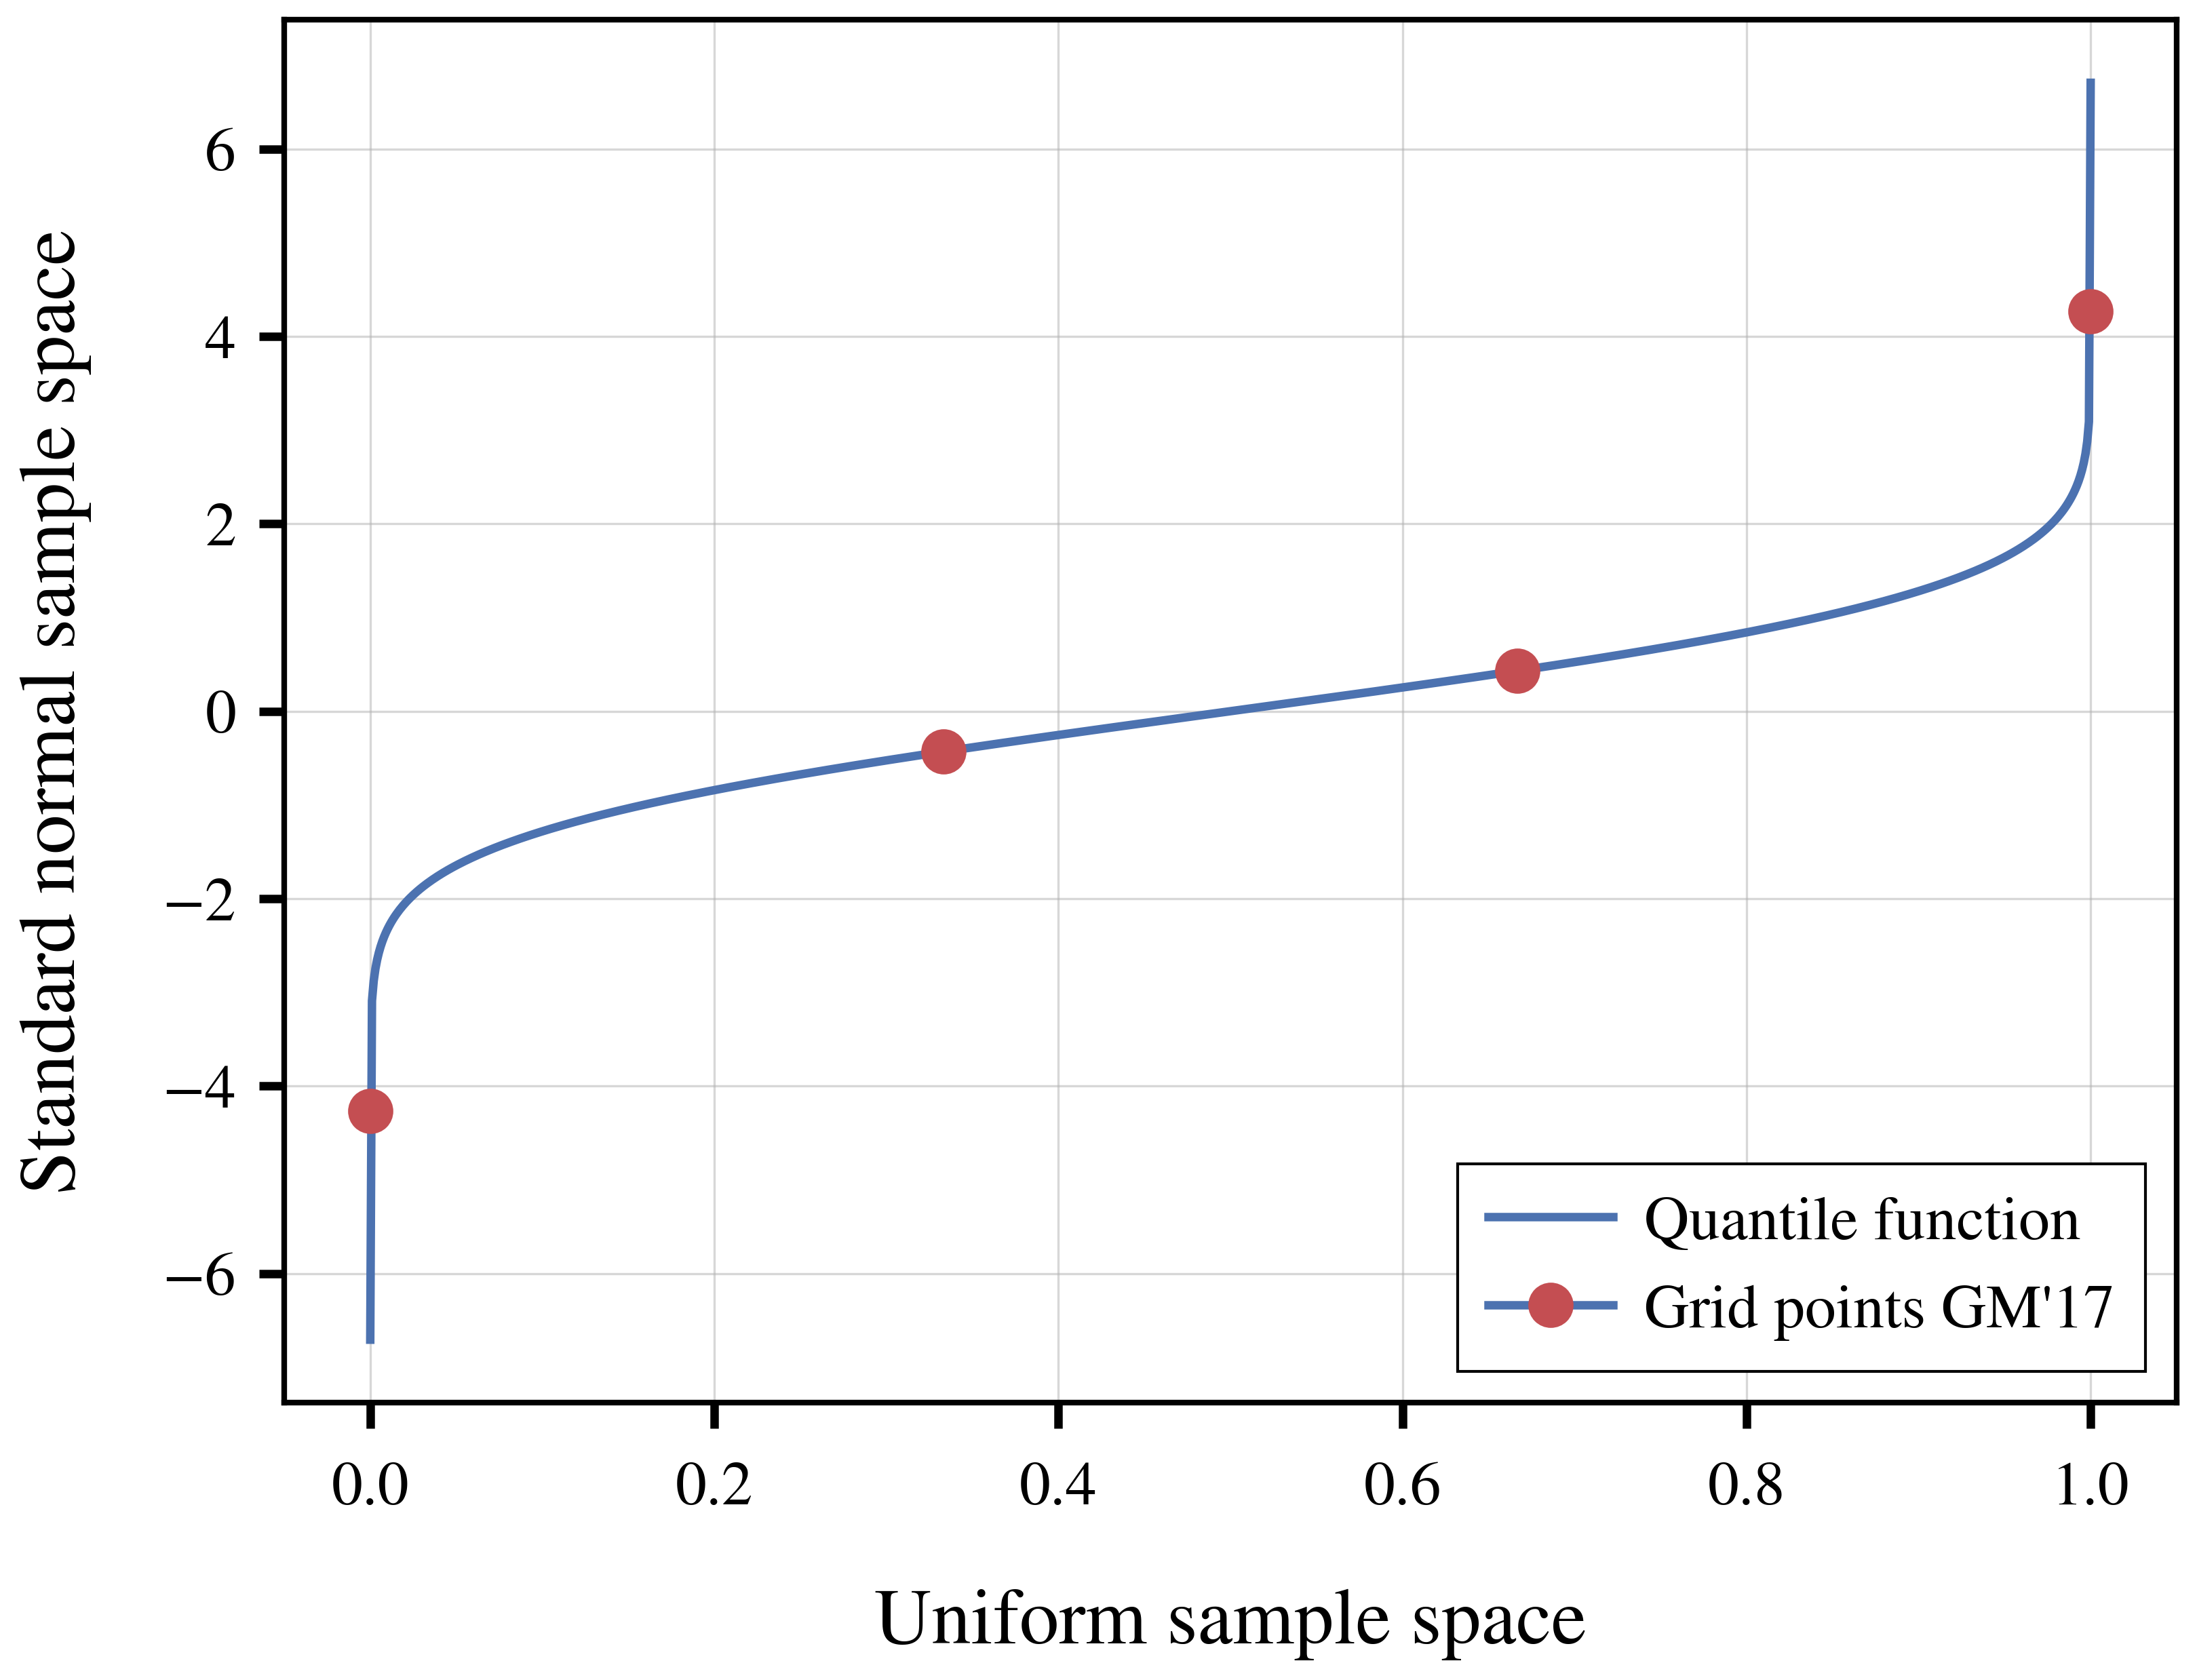
\includegraphics[scale=0.40]{../scrypy/figures/quantile_fct}
	\label{fig:invcdf}
\end{figure}



\begin{figure}[H]
	\captionsetup{format=hang}
	\caption[Comparison of uncertain shares of occupation decisions]{Comparison of shares of occupation decisions over time between scenarios including 99$\%$ confidence intervals}
	\centering
	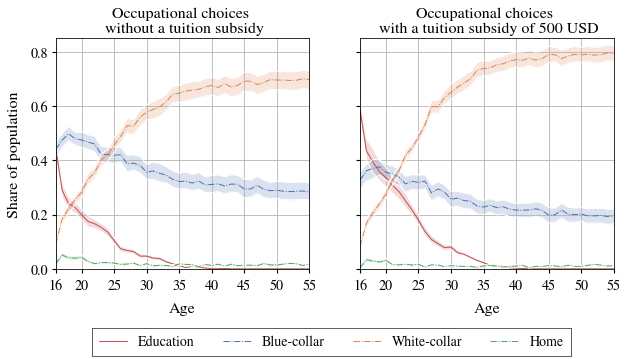
\includegraphics[scale=0.75]{../scrypy/figures/cone_plot_choice_shares}
	\label{fig:uq_paths}
\end{figure}

\vspace{10mm} %5mm vertical space

\begin{figure}[H]
	\caption{Probability distribution of QoI $Y$}
	\centering
	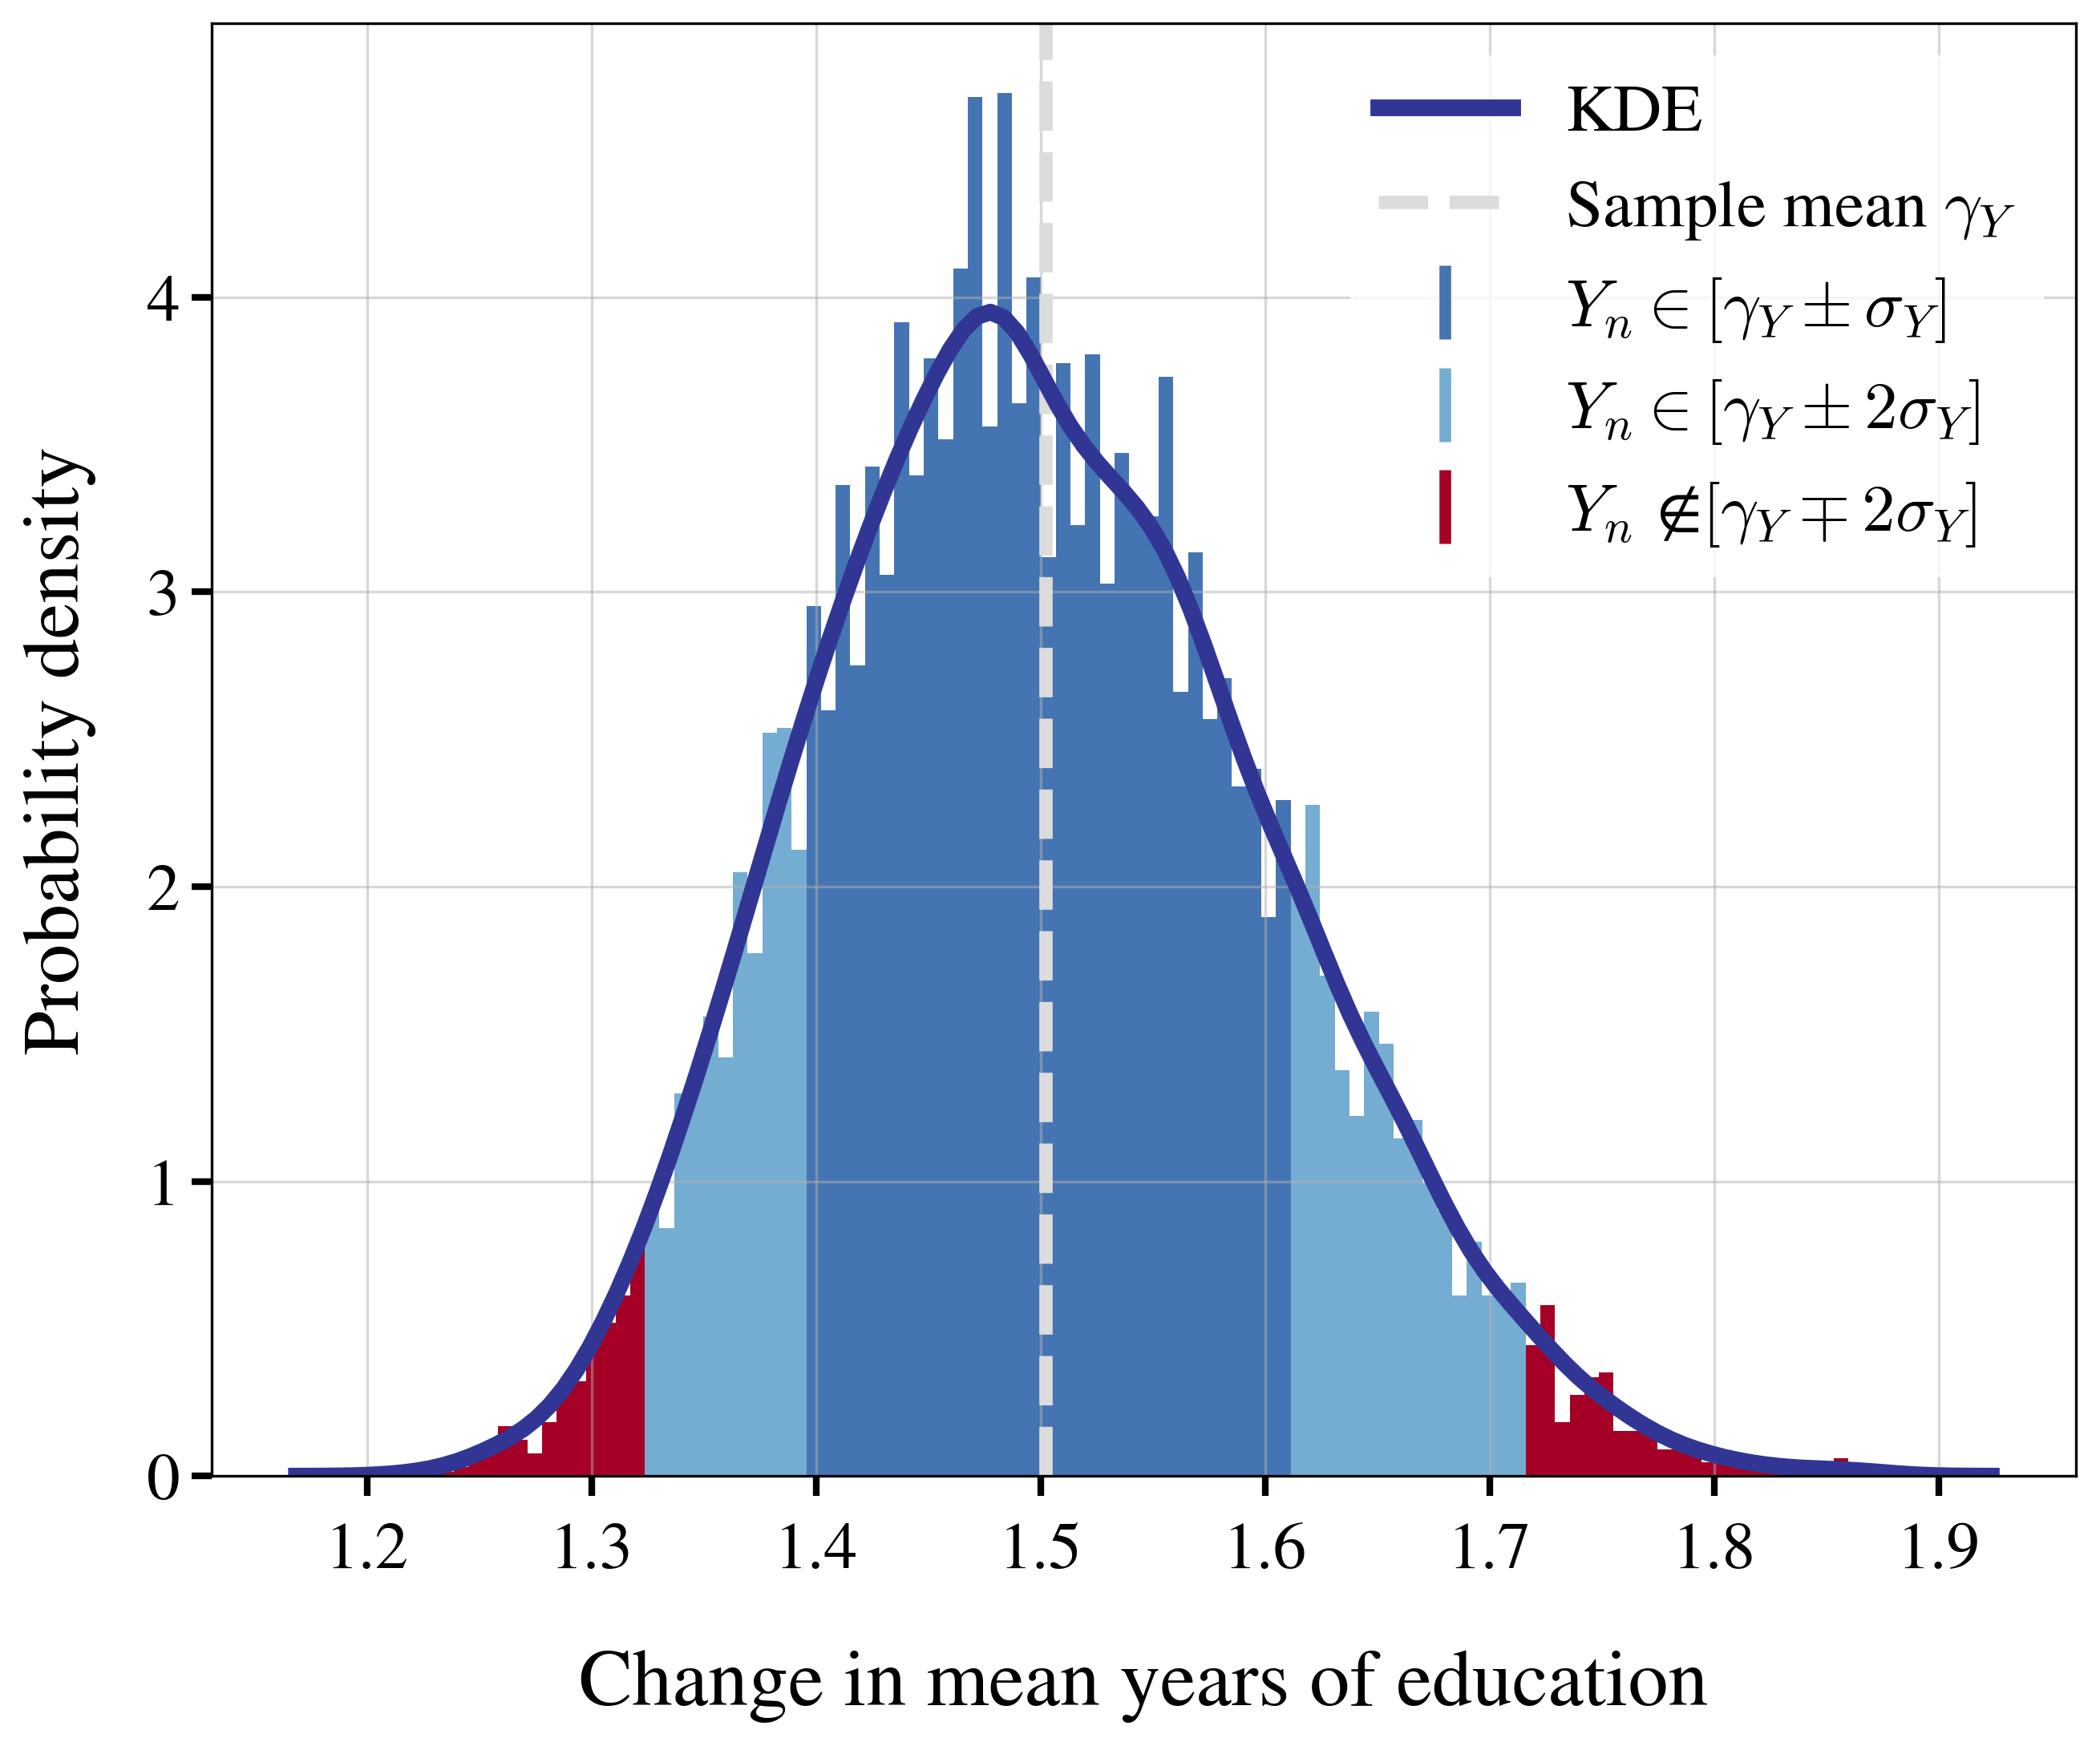
\includegraphics[scale=0.55]{../scrypy/figures/distplot}
	\label{fig:dist}
\end{figure}

\begin{figure}[H]
	\caption[Sigma-normalized mean absolute EEs for radial design]{Sigma-normalized mean absolute Elementary Effects for radial design}
	\centering
	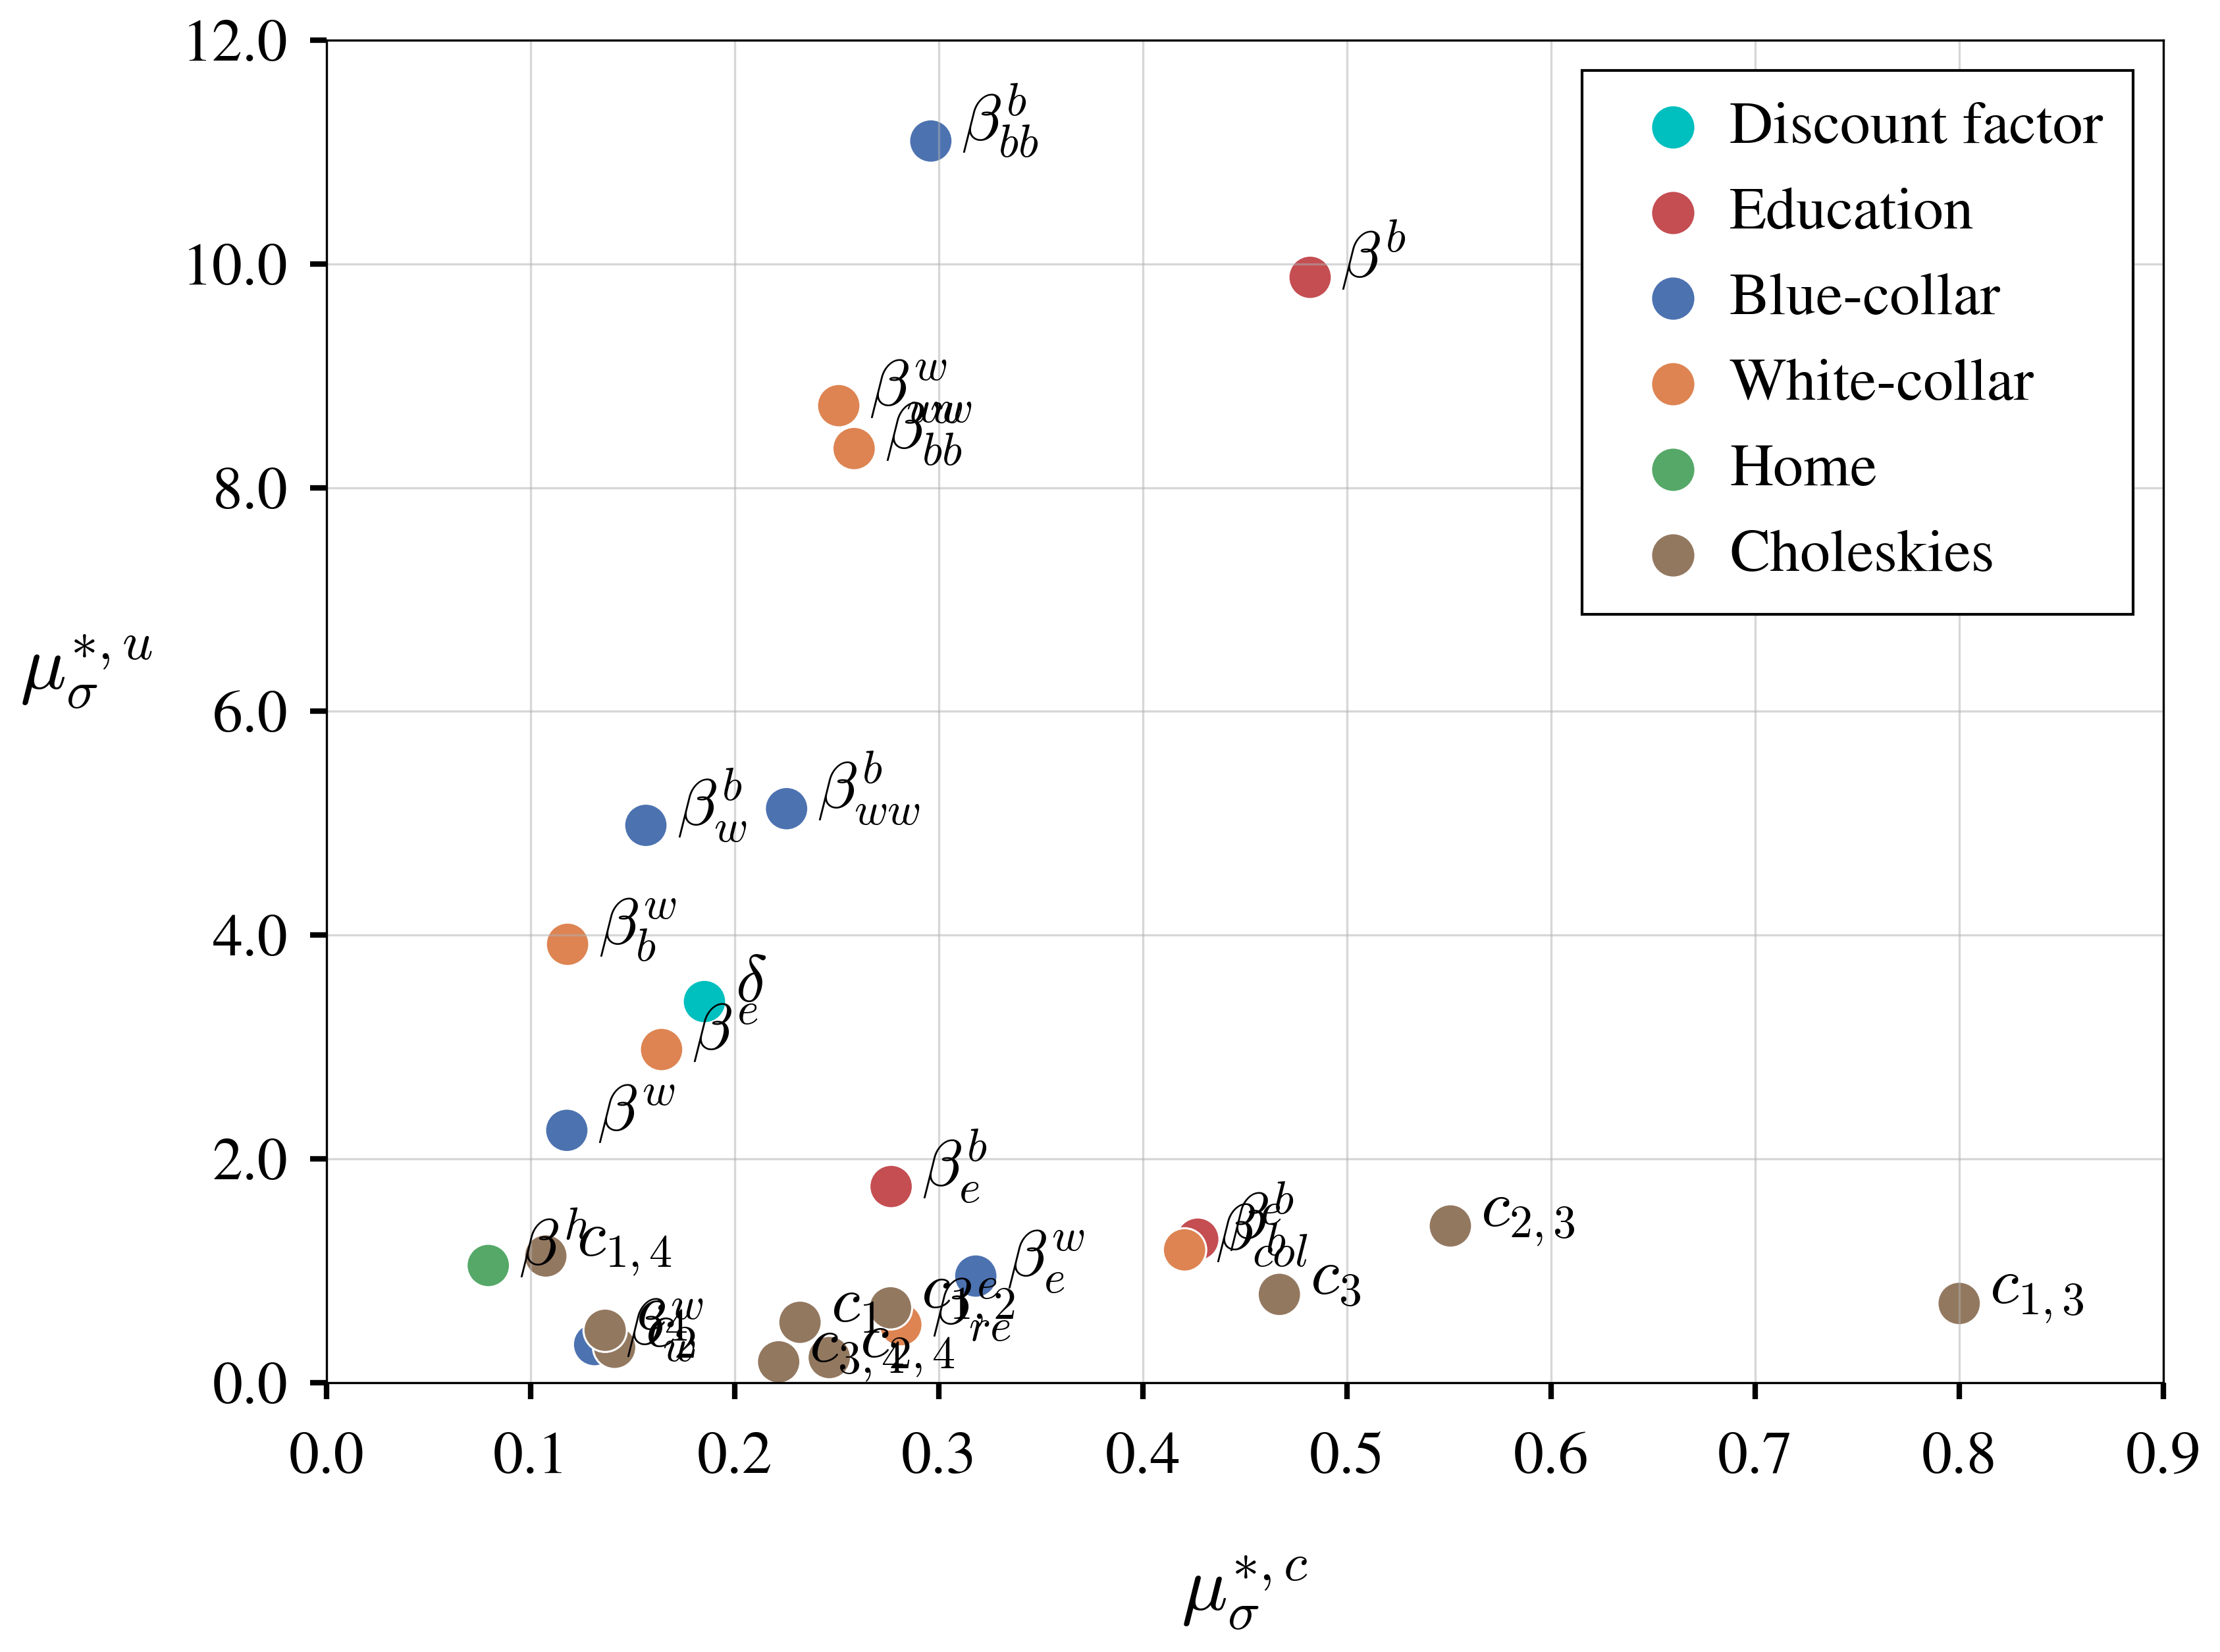
\includegraphics[scale=0.52]{../scrypy/figures/scatter_rad}
	\label{fig:rad}
\end{figure}


\begin{figure}[H]
	\caption[Sigma-normalized mean absolute EEs for trajectory design]{Sigma-normalized mean absolute Elementary Effects for trajectory design}
	\centering
	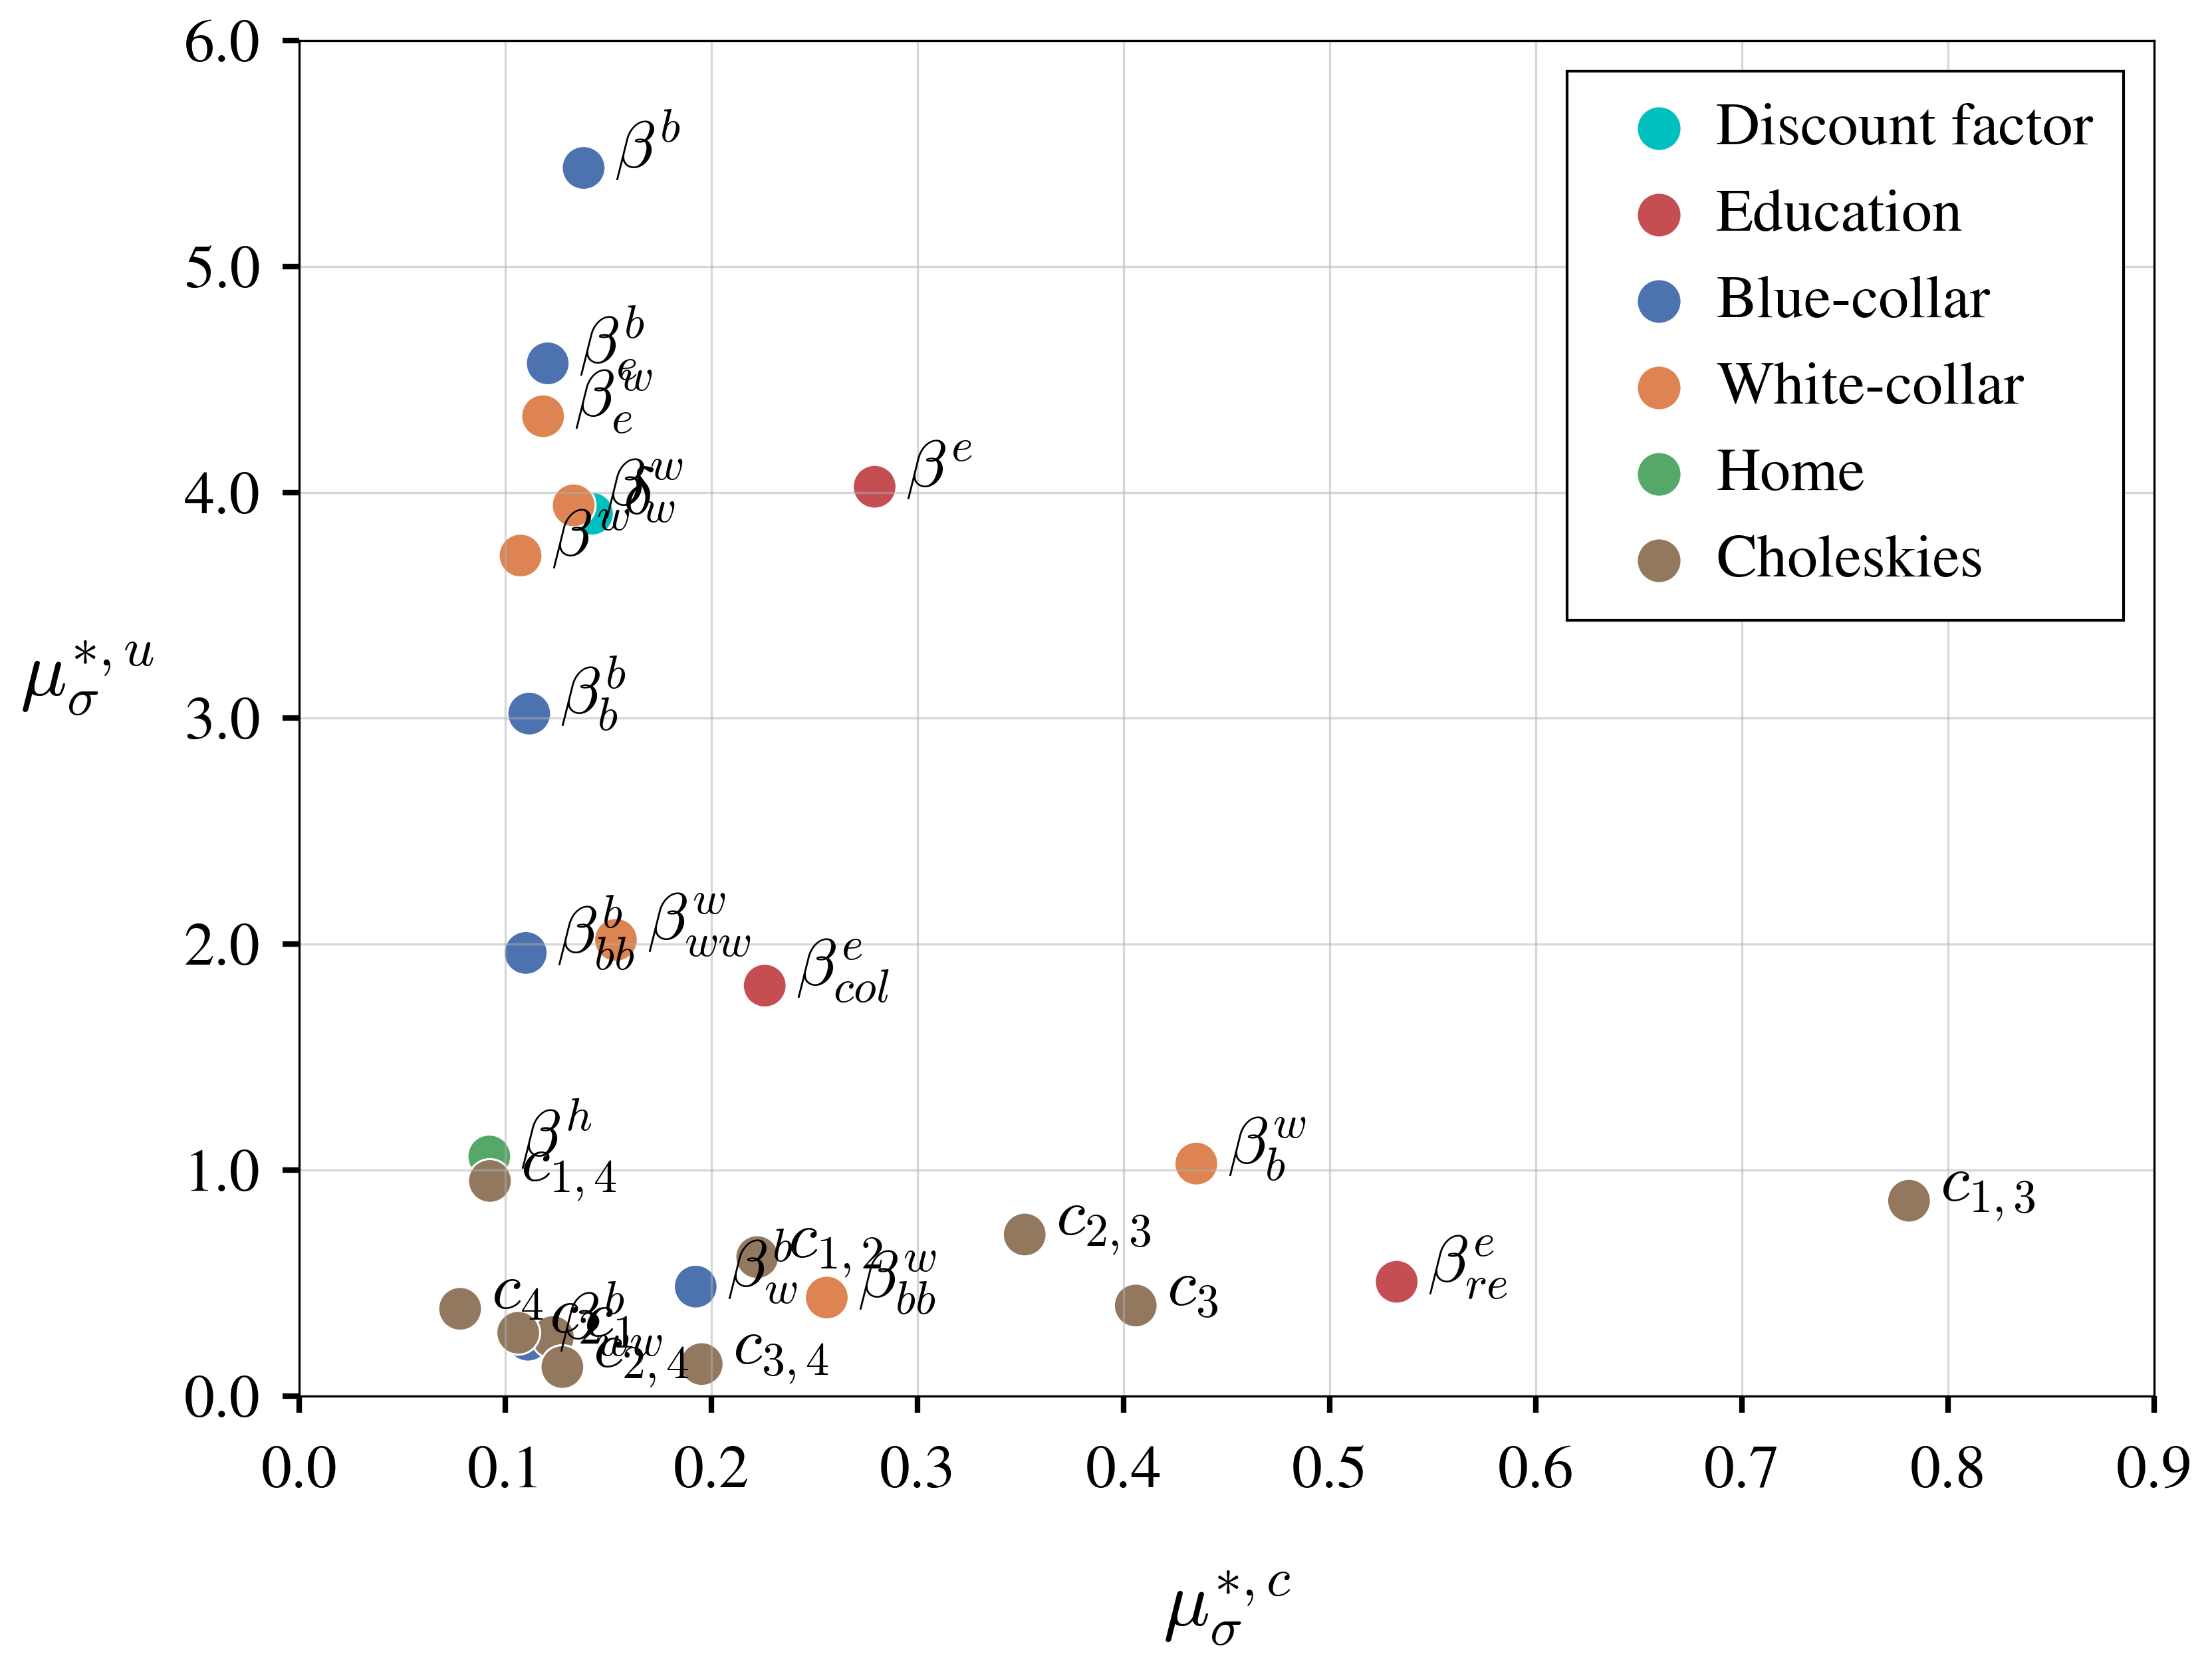
\includegraphics[scale=0.52]{../scrypy/figures/scatter_traj}
	\label{fig:traj}
\end{figure}
\newpage


\subsection{Appendix C: Simulated maximum likelihood estimation}
\thispagestyle{plain} % surpress header on first page
To estimate the exogenous model parameters, the approach that this thesis and also KW94 use is the simulated maximum likelihood method (\cite{Albright.1977})\footnote{See \cite{Aguirregabiria.2010}, p. 42-44 and \cite{Raabe.2019}, p. 21-26 for more details.}.

This method can be applied to a set of longitudinal data on occupational choices $a_t$ and, if available, wages $W_{a,t}^{-}$ of a sample of $i \in I$ individuals starting from age 16. To distinguish from its functional form, let $\mathcal{W}^{-}_{a(k),t}$ denote the measured wages. For each period $t$, the recorded choices $a_0$, ..., $a_{t-1}$  imply the occupation-specific experiences $x_{a,t}$. Together with $t$, they constitute the observable state vector $\bold{s_t^-}$. Consequently, the measured, observable endogenous variables are $\pmb{\mathcal{D}}\defeq(\bold{s_t^-},\mathcal{W}^{-}_{a,t})$. Given this setup, the goal is to estimate the exogenous model parameters $\pmb{\theta}\defeq(\delta, \pmb{\beta}, \pmb{\Sigma_\varepsilon})$.\footnote{Improvements in this thesis' estimation over KW94 are that, first, it is not assumed that the standard errors of the parameters estimates are uncorrelated, and, second, that $\beta$ is not left out of the estimation.} Thus, every probability is a function of the exogenous model parameters $\pmb{\theta}$.
The approach to compute the likelihood function $L_{\pmb{\mathcal{D}}}(\pmb{\theta})$ of the observables in the data begins with the individual latent variable representation in period $t$. The optimal choice is given by
\begin{align}
a_t = \argmax_a V(\bold{s_t^-},\pmb{\varepsilon_t},a_t),
\end{align}
As $a_t$ and $\bold{s_t^-}$ are known, the next step is to derive the unobservable shocks $\pmb{\varepsilon_t}$ in terms of $a_t$ and $\bold{s_t^-}$. Therefore, write the set of shocks for which the alternative-specific value function $V(\bold{s_t^-},\pmb{\varepsilon_t},a_t(j))$ is higher than the other value functions $V(\bold{s_t^-},\pmb{\varepsilon_t},a_t(k\neq j))$ as
\begin{align}
\pmb{\varepsilon_t}(a_t(j),\bold{s_t^-}) \defeq \{\pmb{\varepsilon_t}|V(\bold{s_t^-},\pmb{\varepsilon_t},a_t(j)) = \max_{a_t} V(\bold{s_t^-},\pmb{\varepsilon_t},a_t)\}).
\end{align}
Note that the set condition is a function of the unobservable model parameters $\pmb{\theta}$.

Consider first the case of non-working alternatives $a_t(j) \in [e,h]$. The probability of choosing $a_t(j)$ is the probability of set $\pmb{\varepsilon_t}(a_t(j),\bold{s_t^-})$. This probability equals the integral of the probability distribution function $f(\pmb{\varepsilon_t})$ over all elements of set $\pmb{\varepsilon_t}(a_t(j),\bold{s_t^-})$ with respect to $\pmb{\varepsilon_t}$. Formally,
\begin{align}
\text{p}\big(a_t(j) | \bold{s_t^-}\big) = \int_{\pmb{\varepsilon_t}(a_t(j),\bold{s_t^-})} f(\pmb{\varepsilon_t}) d^{|A|} \pmb{\varepsilon_t}.
\end{align}
\noindent
The second case is $a_t(k) \in [b,w]$. Assuming the dataset contains wages for the working alternatives $a_t(k)$, the probabilities of choosing $a_t(k)$ take a few steps more to compute. First, note from the wage equations that the alternative-specific shocks $\pmb{\varepsilon_{a,t}}$ are normally distributed. Second, in contrary to the non-working alternatives, using (\ref{eq:returns_b_w}), the shocks can directly be expressed as a function of the alternative-specific model parameters $\pmb{\beta_{a(k)}}$ by inserting the inferred alternative-specific experiences $\pmb{x_{a(k),t}}$ into $W_{a(k),t}$ and subtracting the expression from the observed wage $\mathcal{W}^{-}_{a(k),t}$ for each individual. Both wages are logarithmized. Thus,
\begin{align} \label{eq:epsilon}
\varepsilon_{a(k),t} = \text{ln}(\mathcal{W}^{-}_{a(k),t}) - \text{ln}(W_{a(k),t}^{-}).
\end{align}
Third, the alternative-specific shocks $\pmb{\varepsilon_{a,t}}$ are not distributed independently. Since $\varepsilon_{a(k),t}$ can be inferred from the
observed wage $\mathcal{W}^{-}_{a(k),t}$, this information can be used to form the expectation about the whole error distribution. Therefore, using the conditional probability density function $f(\pmb{\varepsilon_t}|\varepsilon_{a(k),t})$, the probability of choosing occupation $a_t(k)$ conditional on observed states and wages writes

\noindent
\begin{align} \label{eq:prob-choice}
\text{p}\big(a_t(k) | \bold{s_t^-},W^{-}_{a(k),t}\big) = \int_{\pmb{\varepsilon_t}(a_t(k),\bold{s_t^-})} f(\pmb{\varepsilon_t}|\varepsilon_{a(k),t}) d^{|A|} \pmb{\varepsilon_t}.
\end{align}
Applying integration by substitution yields the following expression for the probability of the observed wage:\footnote{See \cite{Raabe.2019}, p. 29, 39-40 for a complete derivation.}
\begin{align} \label{eq:prob-wage}
\text{p}\big(\mathcal{W}^{-}_{a(k),t} | \bold{s_t^-}\big) = \omega_t^{-1} \frac{1}{\sigma_{a(k)}} \phi\bigg(\frac{\varepsilon_{a(k),t}}{\sigma_{a(k)}}\bigg).
\end{align}
Here, $\omega_t^{-1}$ is the Jacobian of the transformation from observed wage $\mathcal{W}^{-}_{a(k),t}$ to error $\varepsilon_{a(k),t}$ in (\ref{eq:epsilon}) and $\phi$ is the standard normal probability density function.
Finally, the joint probability of observing choice $a_t(k)$ and wage $\mathcal{W}^{-}_{a(k),t}$ conditional on the observed states is given by the product of the two probabilities in (\ref{eq:prob-choice}) and (\ref{eq:prob-wage}):
\begin{align}
\text{p}\big(a_t(k),\mathcal{W}^{-}_{a(k),t}|\bold{s_t^-}\big) = \text{p}\big(a_t(k)|\bold{s_t^-}, \mathcal{W}^{-}_{a(k),t}\big)\text{p}\big(\mathcal{W}^{-}_{a(k),t}|\bold{s_t^-}\big).
\end{align}
Based on these results, the likelihood contribution $L^{i}_{\pmb{\mathcal{D}}}$ of one individual $i$ can be written as the product of the probability to observe the measured endogenous variables for one individual and for one period over all time periods:
\begin{align}
L^{i}_{\pmb{\mathcal{D}}}(\pmb{\theta}) = P\big(\{a_{t,}^{i},\mathcal{W}^{-,i}_{a,t,}\}_{t=0}^T\big) = \prod_{t=0}^{T} \text{p}\big(a_t^{i},\mathcal{W}_{a,t}^{-,i}|\bold{s_t^{-,i}}\big).
\end{align}
Therefore, the sample likelihood is given by the product of the individual likelihoods over the whole sample of individuals:
\begin{align} \label{eq:sample-likelihood}
L_{\pmb{\mathcal{D}}}(\pmb{\theta}) = P\big(\big\{\{a_{t,}^{i},\mathcal{W}^{-,i}_{a,t,}\}_{t=0}^T\big\}_{i \in I}\big) = \prod_{i \in I}\prod_{t=0}^{T} \text{p}(a_t^{i},\mathcal{W}_{a,t}^{-,i}|\bold{s_t^{-,i})}.
\end{align}
Since the probabilities are functions of the exogenous parameters $\pmb{\theta}$, the simulated maximum likelihood estimator $\pmb{\hat{\theta}}$ is the vector of exogenous parameters that maximizes (\ref{eq:sample-likelihood}). As the maximum likelihood estimator can be shown to be asymptotically normal under some regularity conditions\footnote{This property is an advantage of this thesis' estimation approach. It facilitates the uncertainty quantification via Monte Carlo sampling because there is a simple closed form for the (marginal) probability density available. This eases the construction of the desired samples.}, these results are taken as the mean vector for the input parameters in the uncertainty quantification.

The procedure to estimate the parameter vector $\pmb{\theta}$ using the expressions for the likelihood is as follows: first, The optimization algorithm of choice proposes a parameter vector. Second, the model is solved via backward induction. Third, using the policy functions, the likelihood is computed. These steps are repeated until the optimizer has found the parameter vector that yields the maximal likelihood.\\
\newline
Finally, the calculation of the estimator's covariance is described.\footnote{See \cite{Verbeek.2012}, p. 184-186.} The result is used as the covariance matrix for the input parameters in the UQ.

Under regularity conditions, the asymptotic covariance of a maximum likelihood estimator equals the inverse of the Fisher information matrix $\mathcal{I}(\theta)^{-1}$: $\text{Var}(\theta)=\mathcal{I}(\theta)^{-1}$. In this thesis, the information matrix $\mathcal{I}(\pmb{\theta})$ is given by the variance of the scores of the parameters.\footnote{The computation of $\text{Cov}(\pmb{\theta})$ by using the Jacobian of the individual likelihood contributions is chosen over other approaches because, first, it yields no error in the inversion step of $\mathcal{I}(\pmb{\theta})$ and, second, the results are reasonably close to the similar specification in KW94.} The scores $\text{s}(\pmb{\theta})$ are the first derivatives of the likelihood function. This can be written in terms of sample and individual likelihoods. Formally, the relationships are given by
\begin{align} \label{eq:scores}
\text{s}(\pmb{\theta}) \defeq \frac{\partial L_{\pmb{\mathcal{D}}}({\pmb{\theta}})} {\partial \pmb{\theta}} = \sum_{i \in I} \frac{L_{\pmb{\mathcal{D}}}^{i}(\pmb{\theta})}{\partial \pmb{\theta}} \defeq \sum_{i \in I}\text{s}_i(\pmb{\theta}).
\end{align}
Having multiple individual likelihood contributions, the scores are in the form of the  Jacobian matrix.
Using the property that the expected values of scores, $\E[\text{s}(\theta)]$, are zero at the maximum likelihood estimator. The variance of the scores is given by (\ref{eq:info-matrix}). It is equal to the inverse of the Fisher information matrix.
\begin{align} \label{eq:info-matrix}
\mathcal{I}^{-1}(\pmb{\theta}) = \text{Var}(\text{s}(\pmb{\theta})) = \E[\text{s}(\pmb{\theta})\text{s}(\pmb{\theta})'].
\end{align}
Hence, the estimator for the asymptotic covariance of the maximum likelihood estimator can be written as
\begin{align} \label{eq:est-cov}
\hat{\text{Cov}_J}(\pmb{\hat{\theta}}) = \bigg( \frac{1}{|I|} \sum_{i \in I} \text{s}_i(\pmb{\hat{\theta}})\text{s}_i(\pmb{\hat{\theta}})' \bigg)^{-1},
\end{align}
where $|I|$ is the number of individuals contained in the data set.
The intuition behind the above expression is the following: Estimator $\pmb{\hat{\theta}}$ maximizes the sample likelihood. This is equivalent to $\pmb{\hat{\theta}}$ setting the sample scores to zero. However, the individual likelihood may not be zero at the optimal parameter vector for the sample likelihood. This variation is captured by the variance of the individual scores evaluated at $\pmb{\hat{\theta}}$. The relations in (\ref{eq:scores}) and (\ref{eq:info-matrix}) then imply that the inverse of the variance of the individual scores is equivalent to the variance of the maximum likelihood estimator.

\newpage
\thispagestyle{empty} % e.g. no page number
\section*{Affidavit}
\vspace*{1.0cm}
"I  hereby confirm that the  work  presented  has  been  performed  and interpreted solely by myself except for where I explicitly identified the contrary. I assure that this work has not been presented in any other form for the fulfillment of any other degree or qualification. Ideas taken from other works in letter and in spirit are identified in every single case."\\
\newline
\newline
\newline

\noindent

\rule{5.5cm}{0.4pt} \phantom{ssssssssssssssssspace} \rule{5.5cm}{0.4pt}\\
\phantom{space}Place, Date \phantom{sssssssssssssssssssssssssssssssssssssspace} Signature



\end{document}
